% This is samplepaper.tex, a sample chapter demonstrating the
% LLNCS macro package for Springer Computer Science proceedings;
% Version 2.21 of 2022/01/12
%
\documentclass[runningheads]{llncs}
%
\usepackage[T1]{fontenc}
% T1 fonts will be used to generate the final print and online PDFs,
% so please use T1 fonts in your manuscript whenever possible.
% Other font encondings may result in incorrect characters.
%
% Used for displaying a sample figure. If possible, figure files should
% be included in EPS format.
%
% If you use the hyperref package, please uncomment the following two lines
% to display URLs in blue roman font according to Springer's eBook style:
%\usepackage{color}
%\renewcommand\UrlFont{\color{blue}\rmfamily}
%

%%%%%%%%%%%%%%%%%%%%%%%%%%%%SELF DEFINED AND INPUTS%%%%%%%%%%%%%%%%%%%%%%%%%%%%%%%%%%%%%%%%%%

\usepackage[T1]{fontenc}
\usepackage[normalem]{ulem}
\usepackage{mathtools}
\usepackage{blkarray,bigstrut} 
\usepackage{graphicx,wrapfig,lipsum}
\usepackage{tcolorbox}
\usepackage{enumitem}
\usepackage{array}
\usepackage{algorithm}
\usepackage{algorithmic}
\usepackage{mathpartir}
\usepackage{multirow}
\usepackage{hyperref}
\usepackage{amssymb}
\usepackage{subcaption}
\usepackage{stmaryrd}
\usepackage{color} 


\usepackage{tikz}
\usetikzlibrary{snakes}
\usetikzlibrary{svg.path} 
\usetikzlibrary{calc} 
\usetikzlibrary{shapes}
\usetikzlibrary{shapes.geometric}
\usetikzlibrary{arrows.meta}
\usetikzlibrary{arrows}
\usetikzlibrary{decorations.text,decorations.markings}
% % % % 

%%%%%%%%%%Packages for adaoption%%%

% \usepackage{amsthm} 

%Packages

\input{ldefs}
\newcommand{\highlight}[1]{\textcolor[rgb]{.0,0.0,1.0}{ #1}}
\newcommand{\THESYSTEM}{\textsf{PsRB}}

%%%%%%%%%%%%%%%%%%%%%%%%%%%%SELF DEFINED AND INPUTS%%%%%%%%%%%%%%%%%%%%%%%%%%%%%%%%%%%%%%%%%%

\begin{document}
%
\title{Path Sensitive Reachability Bound Analysis}
%
%\titlerunning{Abbreviated paper title}
% If the paper title is too long for the running head, you can set
% an abbreviated paper title here
%
%%%%%%%%%%%%%%%%%%%%%%%%%%%%Authors%%%%%%%%%%%%%%%%%%%%%%%%%%%%%%%%%%%%%%%%%%
% \author{First Author\inst{1}\orcidID{0000-1111-2222-3333} \and
% Second Author\inst{2,3}\orcidID{1111-2222-3333-4444} \and
% Third Author\inst{3}\orcidID{2222--3333-4444-5555}}
% %
% \authorrunning{F. Author et al.}
% % First names are abbreviated in the running head.
% % If there are more than two authors, 'et al.' is used.
% %
% \institute{Princeton University, Princeton NJ 08544, USA \and
% Springer Heidelberg, Tiergartenstr. 17, 69121 Heidelberg, Germany
% \email{lncs@springer.com}\\
% \url{http://www.springer.com/gp/computer-science/lncs} \and
% ABC Institute, Rupert-Karls-University Heidelberg, Heidelberg, Germany\\
% \email{\{abc,lncs\}@uni-heidelberg.de}}
%
%%%%%%%%%%%%%%%%%%%%%%%%%%%%Authors Above%%%%%%%%%%%%%%%%%%%%%%%%%%%%%%%%%%%%%%%%%%

\maketitle              

% typeset the header of the contribution
%
\begin{abstract}
\todo{150--250 words.}
Goal: bound the number of visiting times for every program control location, i.e., Solve the 
\emph{Reachability-Bound Program}.
\\
Motivation: State-of-Art Techniques 
\\
in paper~\cite{Sumit2010rechability,sinn2017complexity} : path-insensitive 
\\
in paper~\cite{GulwaniJK09} : path-sensitive and precise for estimating loop bounds,
but over-approximate reachability times of control location as the loop bound.
\\
in paper~\cite{ZulegerGSV11} : able to identify different paths from multiple-path loop, but aims to solve bounds for loop and path. They over-approximate reachability times of control location with loop bound.
\\
Contributions: 
\\
1. Solve the 
\emph{Reachability-Bound Program} precisely /(improve accuracy),
in two challenging classes of programs: Programs with Path-Sensitive Loops, and Programs with Nested Loops 
\\
2. Improved efficiency by abstracting program using the Difference Constraint-base method in \cite{sinn2017complexity}.
\\
3. Efficient implementation and evaluation results.
\keywords{Loop Bound Inference, program refinement, path-sensitive}
\end{abstract}
%
%
%
%%%%%%%%%%%%%%%%%%%%%%%%%%%%%%%%%%%%%%%%%%%%%%%%%%%%%%%%%%%%%%%%%%%%%%%%%%%%%%%%%%%%%%%%%%%%%%%%%%%%%%%%%%%%%%%%%%%%%%%%%%%%%%%%%%%%%%%%%
%%%%%%%%%%%%%%%%%%%%%%%%%%%%%%%%%%%%%%%%%%%%%%%% The Introduction and Overview %%%%%%%%%%%%%%%%%%%%%%%%%%%%%%%%%%%%%%%%%%%%%%%%%%%%%%%%
%%%%%%%%%%%%%%%%%%%%%%%%%%%%%%%%%%%%%%%%%%%%%%%%%%%%%%%%%%%%%%%%%%%%%%%%%%%%%%%%%%%%%%%%%%%%%%%%%%%%%%%%%%%%%%%%%%%%%%%%%%%%%%%%%%%%%%%%%
\section{Introduction}
\label{sec:intro}

Gulwani et. al~\cite{GulwaniZ10} first introduce \emph{reachability-bound} as the upper bound on the number of times a given control location 
inside a procedure is visited during program execution.
A tight reachability-bound has many applications.
For example from a privacy and security perspective,
how much secret information is leaked by a program depends on the number of times a certain operation that leaks the data
is executed~\cite{Malacaria07};
from an efficiency perspective, when different program locations consume different resources, a precise reachability-bound of each location can help to estimate the resource cost more accurate than just computing the overall complexity.
While existing works all have different limitations when inferring the \emph{reachability-bound}.
For example, Gulwani et. al~\cite{GulwaniZ10}
give a two-step solution by combining program abstract and proof-rules-based bound computation.
But it does not compute the \emph{reachability-bound} precisely for every control location.
Instead, they only compute the complexity bounds for overall loop and over-approximate for different locations using this bound,
which is loose especially when there are multipath loops.
Techniques in program complexity analysis~\cite{GustafssonEL05,HumenbergerJK18} 
or worst-case resource cost analysis
~\cite{BrockschmidtEFFG16,AlbertAGP08,AliasDFG10,Flores-MontoyaH14} can be repurposed to estimate similar quantities such as the
bounds on loop iterations, execution time, etc.
While these quantities focus only on  
the overall complexity,
none of them compute the reachability-bound on a given program control location directly or path-sensitively.
This leads to inaccuracy in data leakage analysis, resource cost estimation, etc.
To overcome these limitations, 
we introduce a novel path-sensitive reachability-bound analysis algorithm that solve 
the reachability-bounds problem efficiently and path-sensitively.
It is built over an abstract transition graph which effectively combines amortized complexity analysis with loop summarization based multipath refinement.
This combination mitigates the limitations faced by either technique individually. 
Before diving into the algorithm, below are some related works and their limitations.

% \begin{itemize}
% \item 
\emph{Program Abstraction.}
Program abstraction is commonly used in program analysis as a preprocessing step to abstract program features and generate transition graphs or systems. For example, Gulwani et. al~\cite{GulwaniZ10} summarizes programs into some underlying abstract domains (the unified lattice~\cite{CousotH78}, polyhedra~\cite{CousotC77} or octagonal~\cite{Mine06})
and generates transition systems for loop counters.
\cite{KincaidCBR18} abstracts program into the wedge domain and computes the non-linear loop invariant.
%  While it only works well for the specific targeting problem.
Efficiency is the main bottleneck when generating and solving the constraint.
We choose to use the difference constraint based program abstraction model~\cite{SinnZV17,SinnZV14} combined with boolean expression to generate our abstract transition graph.
It is more accurate in the sense of representing the program loops path-sensitively. This representation is also comparatively lightweight.

% \item 
\emph{Amortized Complexity Analysis.}
One line of complexity analysis follows the idea of the \emph{amortized complexity analysis}
originated from Tarjan's influential paper~\cite{PotechinP17}. It is usually combined with ranking functions~\cite{BradleyMS05,CookSZ13,Zuleger18} or counter increments~\cite{ZulegerGSV11,SinnZV14,SinnZV17,LuCT21,AliasDFG10}.
They do well in nested loops by alternating the loop bound computation with the ranking or counter estimation. This alternation is efficient without recursively unrolling the nested loops when composing the bound of different paths.
  % \\
  But estimating the counter or ranking function invariant ignores the interleaving between multiple paths in the same loop,
% Most of them 
such as the tools CofloCo~\cite{Montoya17,Flores-MontoyaH14,Flores-Montoya16}, KoAT~\cite{BrockschmidtEFFG16,BrockschmidtEFFG14,FalkeKS12,FalkeKS11}, the algorithm in~\cite{LuCT21}, and etc.
%  over-approximate the loop bound when the path interleaving affects loop execution.
It is hard to repurpose their result as the reachability-bound on different points.
% loop bound path-insensitively as the reachability-bound on different points.
Another kind of \emph{amortized complexity analysis} based on type refinement or annotation~\cite{CraryW00,JostHLH10,CicekBG0H17,RajaniG0021,CarbonneauxHS15} has the same weakness in the multipath loops, resulting in the over-approximation of the resource cost on different program points.
To overcome these limitations, we enrich it with path-sensitivity according to the Alg.~2 in~\cite{SinnZV14},
% which assigns a variable to each edge on which this variable decrease as its ranking function.
the Alg.~3 in~\cite{ZulegerGSV11},
and the Def.~25 in Section 4 from~\cite{SinnZV17}.

\emph{Loop Summarization and Path Refinement Based Complexity Analysis}.
Another line of loop bound analysis through loop summarization and path refinement seeks for precise loop path representation~\cite{ManoliosV06,BalakrishnanSIG09,SharmaDDA11,Flores-MontoyaH14,HumenbergerJK18,CyphertBKR19}, and explicating the interleaving between paths~\cite{GulwaniJK09,ZulegerGSV11}.
\cite{KincaidBCR19,KincaidCBR18,BreckCKR20} introduce some loop summarization techniques which can help to improve the accuracy of the path refinement but specifically for non-linear loops, program recurrence, etc.
%  summarization techniques~\cite{KincaidCBR18} and the invariant generating algorithm considering recurrence in~\cite{BreckCKR20}. 
However, when composing the bound between nested loops, recursively unrolling the nested loops is heavy and non-terminating in most cases.
%
Our method simplifies the path refinement algorithm in~\cite{GulwaniJK09} using contextualization techniques based on~\cite{ZulegerGSV11,SinnZV14,ManoliosV06}.
We also limit the iterations of the refinement algorithm to a constant in our bound analysis algorithm.
% \end{itemize}
%

We perform both path refinement and ranking estimation over an abstract transition graph through program abstraction presented in Section~\ref{sec:progabs}.
This combination utilizes the effectiveness of \emph{amortized complexity analysis} by computing the ranking function
% $\locbound(\absevent, c)$ for each transition edge $\absevent$, 
and estimating its bound invariant in Section~\ref{sec:rank}.
It additionally benefits from the accuracy of path refinement techniques through a light-weight path refinement algorithm adopted from~\cite{GulwaniJK09} in Section~\ref{sec:refine}.
Building on this combination, we introduce two novel quantities,
the \emph{path reachability-bound} and \emph{loop reachability-bound}.
The first one bounds the evaluation times of each loop free and interleaving free path in a refined program, and the second one bounds the iterations of an outer loop w.r.t. the innermost loop such that in these iterations of outer loop, the innermost loop is ``entered''. 
Then we present the algorithm for estimating the two quantities in Section~\ref{sec:looprb} and~\ref{sec:pathrb} and compute the \emph{reachability-bound} for each program point path-sensitively in Section~\ref{sec:psrb}.
Our evaluation on the prototype implementation in Section~\ref{sec:eval} shows that we can accurately estimate different bounds for different program points on multiple loop paths. By summing up the different \emph{reachability-bound}s on every location, the results shows a big improvement comparing to the state-of-art worst case complexity analysis.

To recapitulate, our main contributions are summarized as follows.
\\
% \begin{itemize}
%   \item 
1. A path-sensitive reachability-bound algorithm which computes sound bound on the evaluation times of each program point path-sensitively.
\\
%  \item 
2. The combination of \emph{amortized bound analysis} through ranking function estimation and the path refinement approach in our algorithm.
% \item 
\\
3. Two novel quantities, the \emph{path reachability-bound} and \emph{loop reachability-bound} and their corresponding estimating algorithms.
% \item 
\\
4. A prototype implementation with evaluation over four different benchmarks.
  The evaluation shows big improvement comparing to the state-of-art worst case complexity analysis, and potential applications in other areas.
% \end{itemize}
\section{Overview}
\label{sec:overview}
In this section, we discuss a representative running examples with
challenges of analyzing the symbolic
\emph{reachability-bound} on
every control location and illustrate our key novelties, \emph{path reachability-bound} and the \emph{loop reachability-bound}.
This example is adopted from the example in~\cite{GulwaniZ10}, which
is a skeleton code from the .Net base-class library.

% \paragraph{Challenges.}
\begin{example}
  [The Running Example with Two Paths Loop and Nested Loop in One Path]
  \label{ex:relatedNestedWhileOdd_abscfg}
    { \small
  \begin{figure}
  \centering
  \begin{subfigure}{.4\textwidth}
    \begin{centering}
    {\small
    $
    \begin{array}{l}
      \kw{nestedOdd}(n, m) \triangleq \\
      \clabel{ \assign{i}{n} }^{0} ; \\
          \ewhile ~ \clabel{i > 0}^{1} ~ \edo ~ \\
          \qquad \Big(
            \eif(\clabel{i \% 2 \neq 0 }^{2},\\
            \qquad \clabel{\assign{k}{i - m}}^{3};\\
            \qquad \ewhile ~ \clabel{k > 0}^{4} ~ \edo ~
            \Big( \clabel{\assign{k}{k - 1}}^{5} \Big);\\
            \qquad \clabel{\assign{i}{k + m}}^{6};
            \clabel{\assign{i}{i - 1}}^{7}, \\
            \qquad \clabel{\assign{i}{i - 3}}^{8})
            \Big)
      \end{array}
    $
    }
    \caption{}
    \end{centering}
    \end{subfigure}
  \begin{subfigure}{.5\textwidth}
    \begin{centering}
  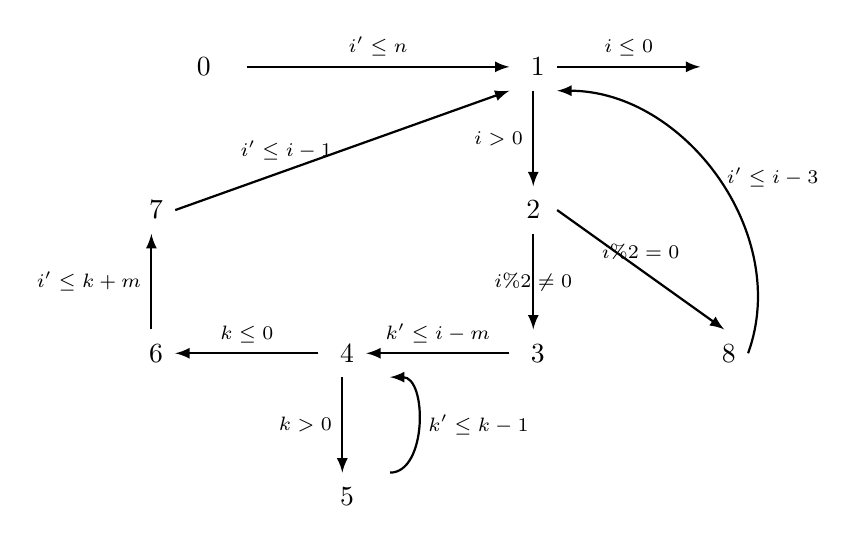
\begin{tikzpicture}[scale=\textwidth/20cm,samples=200]
  \draw[] (-7, 10) circle (0pt) node{{ $0$}};
  \draw[] (0, 10) circle (0pt) node{{ $1$}};
  \draw[] (0, 7) circle (0pt) node{\textbf{$2$}};
  \draw[] (0, 4) circle (0pt) node{{ $3$}};
  \draw[] (-4, 4) circle (0pt) node{{ $4$}};
  \draw[] (-8, 4) circle (0pt) node{{ $6$}};
  \draw[] (-4, 1) circle (0pt) node{{ $5$}};
  \draw[] (4, 4) circle (0pt) node{{ $8$}};
  \draw[] (-8, 7) circle (0pt) node{{ $7$}};
  % Counter Variables
  \draw[] (4.5, 10) circle (0pt) node {\textbf{$\lex$}};
  % \draw[] (6, 4) circle (0pt) node {{ $ex$}};
  %
  % Control Flow Edges:
  \draw[ thick, -latex] (-6, 10)    -- node [above] {\scriptsize $i' \leq n$}(-0.5, 10);
  \draw[ thick, -latex] (0, 9.5)    -- node [left] {\scriptsize $i > 0$} (0, 7.5) ;
  \draw[ thick, -latex] (0.5, 7)    -- node [above] {\scriptsize $ i \% 2 = 0 $}  (4, 4.5);
  \draw[ thick, -latex] (4.5, 4)    to  [out=70,in=0]   node [right] {\scriptsize $i' \leq i - 3$ }(0.5, 9.5);
  \draw[ thick, -latex]  (0, 6.5)   -- node  {\scriptsize $i \% 2 \neq 0$}  (0, 4.5) ;
  \draw[ thick, -latex]  (-0.5, 4)  -- node [above] {\scriptsize $k' \leq i - m$ }  (-3.5, 4) ;
  \draw[ thick, -latex]  (-4.5, 4)  -- node [above] {\scriptsize $k \leq 0$ }  (-7.5, 4);
  \draw[ thick, -latex] (0.5, 10)   -- node [above] {\scriptsize $i \leq 0$}  (3.5, 10);
  \draw[ thick, -latex] (-4, 3.5)   -- node [left] {\scriptsize $k > 0$}  (-4, 1.5);
  \draw[ thick, -latex] (-3, 1.5)   to  [out=0,in=0] node [right] {\scriptsize $k' \leq k- 1$}  (-3, 3.5);
  \draw[ thick, -latex] (-8, 4.5)   --  node [left] {\scriptsize $i' \leq k + m$ }(-8, 6.5);
  \draw[ thick, -latex] (-7.5, 7)  --  node [left] {\scriptsize $i' \leq i - 1$ }(-0.5, 9.5);
  % \draw[ thick, -latex] (6, 6.5)  -- node [right] {$\top$} (6, 4.5) ;
  \end{tikzpicture}
  \caption{}
    \end{centering}
    \end{subfigure}
\begin{subfigure}{.9\textwidth}    
\begin{centering}
  {\small
  $\tpath_0 = (0 \to 1)$
  \quad
  $\tpath_1 = (1 \to 2 \to 3 \to 4)$
  \quad
  $\tpath_2 = (4 \to 6 \to 7 \to 1)$
  \quad
  $\tpath_3 = (4 \to 5 \to 4)$
  \quad
  $\tpath_4 = (1 \to 2 \to 8 \to 1)$
  \quad
  $\tpath_5 = (1 \to \lex)$
  \\
  $
  \tpath_0 ; \rpchoose{ 1: \rprepeat(\tpath_1; 4:\rprepeat(\tpath_3); \tpath_2; \tpath_4), 
  1: \rprepeat(\tpath_4; \tpath_1; 4:\rprepeat(\tpath_3); \tpath_2) }; \tpath_5
  $
  }
  % \caption{}
    \end{centering}
    \end{subfigure}
  \caption{
  (a) The program of the two paths loop with a nested Loop in one path,
    (b) The corresponding \emph{Abstract Transition Graph}, $\absG(\kw{nestedOdd}(n, m))$. }
      \label{fig:relatedNestedWhileOdd-overview}
  \end{figure}
  }
  %
  \end{example}    
  
\footnotetext{We use the notation $(l_0 \to \cdots \to l_n)$ to denote a vertices sequence $(l_0, \cdots, l_n)$, and the constraint on each edge in each transition path are omitted for concise.}
% \todo{Shorten}
% \begin{itemize}
%   \item 
\textbf{Challenge I}
  In this example, given $n \geq m$,
the precise \emph{reachability-bound}s for control locations $4$ and $5$ are both $m \times \lfloor\frac{n}{m}\rfloor$,
for location $2$ and $3$ are $(m + 1) \times \lfloor\frac{n}{m}\rfloor + 1$, 
and $1$ for locations $0, 1$ and $\lex$. 
\highlight{Notice here, though within the same loop $L_2$, the bounds for locations $4$ and $5$ on the first branch, and $6$ on the second branch are different.}
\\
However, the state-of-art \emph{reachability-bound} analysis~\cite{GulwaniZ10}
gives the same \emph{reachability-bound}, $n + \lfloor\frac{n}{m}\rfloor$ for all the locations within the loop $L_2$, which is tight w.r.t. $L_2$'s iteration times but not for different locations inside $L_2$ without considering multiple paths.
Among works on program complexity, cost and loop bound analysis, \cite{GulwaniJK09} can also compute the tight bound on the loop iteration but not reachability-bound on each location path-sensitively.
Though we can use it as the \emph{reachability-bound} for location $1$ and $2$,
the \emph{reachability-bounds} for control locations $4, 5$ and $6$ are still unclear.

This motivates us the first key novelty -- the \emph{path reachability-bound} $\inoutB(\rprog, \tpath)$ for a loop free path $\tpath$ within a loop program $\rprog$ bounds the evaluation times of each loop free path instead of the entire multipath loop.
% \item 

\textbf{Challenge II}
  Then in line 8, $i$ is reset by $w$ and $w$ is reset by $j$ at line 5. So the
while $L_6$ is only executed in the first iteration of while loop $L_1$ and $L_3$.
% \\
The while loop $L_3$ at line 3 is executed only in 
the first $m - N$ iterations of the 
$L_1$ because $j$ is reset by $i$ in line 2.
% \\
So the total iterations of all the three loops is
$n + m^2 - m \times N$,
and the precise \emph{reachability-bound} for location $7$ inside the $L_6$ is $N$,
for locations $4, 5$ and $8$ between the $L_3$ and $L_6$ are $(n-N) \times (m - N)$,
and $n - N$ for locations $2$ and $9$.
% \\
\highlight{Notice here the \emph{reachability-bounds} for the locations inside the loop $L_6$ is 
the same as its innermost loop iteration bound.
% , as well as our \emph{path reachability-bound}.
However, for the locations between $L_3$ and $L_6$,
the \emph{reachability-bounds} are the multiplication of the inner and outer loop iteration bounds.}
\\
To the best of our knowledge, the loop bound analysis method in \cite{GulwaniJK09} can only give a loose bound $n + (m \times n) + N$ for the entire loop complexity, and 
the DC-based algorithm in \cite{SinnZV17} is able to
compute a better but still loose bound, $n + m^2 - m \times N$ on total iteration times.
None of them can give the precise \emph{reachability-bound} for every location in these nested loops,
which is non-trivial to compute even though knowing the loop bound.
% especially for the locations similar to $7$ in $\kw{threeNestedWhile}$.

\highlight{
This motivates use consider our second novel quantity --
the numbers of iterations of the outside loop $L_3$ and $L_1$ such that,
during these iterations, the loop $L_6$ is ``entered''. 
We call this the \emph{loop reachability} of the location within loop $L_6$ w.r.t the loops $L_3$ and $L_1$.
Then by multiplying the loop iteration bound of the $L_6$ with its \emph{loop reachability} times w.r.t the  $L_3$ and $L_1$, we can compute the precise
\emph{reachability-bounds} for location $7$.
}

\highlight{
This quantity isn't considered or computed in any of the previous works.
In the line of methods based on path refinement and loop summarization, the \emph{Progress Invariant} method in \cite{GulwaniJK09} is only able to compute
the
bound on iteration numbers
of the inner loop $L_6$ in each iteration of $L_3$ and $L_1$, which are both $N$.
So they have to over-approximate the reachability-bound for locations inside $L_6$ with the
overall program complexity by multiplication, i.e., $n + m^2 - m \times N$.
In the line of the \emph{amortized complexity analysis} through ranking function, the DC-based algorithm in \cite{SinnZV17}
is only able to
compute the combined loop bound and the local bound of each loop
separately as well.
% We are still unable to know the precise \emph{reachability-bound} for the locations in the innermost loop.
}
% \end{itemize}
With the two key novelties, our algorithm computes the reachability-bound for this example through the following steps.
% \paragraph{Main Steps of Path-sensitive Reachability-bound Analysis}
% \label{sec:static_rb}

\textbf{\emph{Step1: Program abstraction.}}
In Section~\ref{sec:progabs},
we first 
generate the \emph{Abstract Transition Graph} as in Figure~\ref{fig:relatedNestedWhileOdd-overview}(b).
Each edge $l \xrightarrow{dc} l'$ is an abstract transition $\absevent = (l, dc, l')$ annotated with a constraint $dc$ corresponding to the command of label $l$.

Then we abstract the program in the form of paths.
$$
\tpath_0 ; \rpchoose{ 1: \rprepeat(\tpath_1; 4:\rprepeat(\tpath_3); \tpath_2), 1:\rprepeat(\tpath_4) }; \tpath_5
$$
$;$ concatenates sequence of execution paths,
$\rprepeat(\tpath_3)$ represents looping on the path $\tpath_3$ and
$\rpchoose{ \ldots}$ represents the loop $L_1$ which contains two possible execution paths,
$\rprog_1 = \tpath_1; 4:\rprepeat(\tpath_3);\tpath_2$ and $\rprog_2 =\tpath_4$.

% \textbf{Step 2: Program Refinement}
\textbf{\emph{Step 2: Path interleaving refinement.}} 
Two execution paths are not simply iterating on themselves during the program execution,
they could interleave each other at certain iteration.
We summarize each execution path into conjunctions of transition relations.
\begin{equation}
    \begin{array}{l}
        \rprog_1 \models \phi_1 = \\
    \rprog_2 \models \phi_2 = 
    \end{array}
\end{equation}
  
In this sense, Algorithm~\ref{alg:prog-refine} in Section~\ref{sec:refine} computes the interleaving orders
by exhaustively checking the compositions of transition relations of different execution paths,
\begin{equation}
    \begin{array}{l}
        \rprog_1 ; \rprog_1 \models \exists i, k \st \phi_1 \circ \phi_1 = ... \implies \efalse\\
        \rprog_2 ; \rprog_2 \models \exists i, k \st \phi_2 \circ \phi_2 = ... \implies \efalse \\
        \rprog_2 ; \rprog_1 \models \exists i, k \st \phi_2 \circ \phi_1 = ...  \\
        \rprog_1 ; \rprog_2 \models \exists i, k \st \phi_1 \circ \phi_2 = ... 
    \end{array}
\end{equation}
Only two execution paths are feasible, so we identify two unique interleaving orders --
either $\rprog_1$ executes after one iteration of $\rprog_2$ or vice versa.
% Then, loop $L_1$ in the source program is generates new execution paths as follows,
\[
    \rprog^1 = \rprog_1 ; \rprog_2 = \tpath_1; 4:\rprepeat(\tpath_3); \tpath_2; \tpath_4
    \qquad
    \rprog^2 = \rprog_2 ; \rprog_1 = \tpath_4; \tpath_1; 4:\rprepeat(\tpath_3); \tpath_2
\]
% The second step in Section~\ref{sec:refine}
Then, the multiple-paths loop $L_1$ in the source program is refined
into multiple loops where each one can only iterate following the specified interleaving order.
% the interleaving of paths is explicit.
As in the bottom of Figure~\ref{fig:relatedNestedWhileOdd-overview}(c),
the program is transformed into 
\[
    \tpath_0 ; \rpchoose{ 1: \rprepeat(\tpath_1; 4:\rprepeat(\tpath_3); \tpath_2; \tpath_4), 
1: \rprepeat(\tpath_4; \tpath_1; 4:\rprepeat(\tpath_3); \tpath_2) }; \tpath_5
\]
In this refined program, 
each new execution path is equivalent to the execution of the original loop. 
% denoted as $\rprog_1^1$ and $\rprog_1^2$.

% \textbf{Step 3: Ranking Function Estimation}
\textbf{\emph{Step 3: ranking function estimation.}}
Algorithms in Section~\ref{sec:rank} identifies the ranking function for each transition edge, which is a symbol whose number of decreasing times can represent the number of execution of this edge.
For example for edge $4 \to 5$, its ranking function is $k$ and edges on $\tpath_1$, $\tpath_2$ and $\tpath_4$ all have $i$ as their ranking functions.

% \textbf{Step 4: Path-sensitive Reachability-bound Computation.}
\textbf{\emph{Step 4: local path reachability-bound.}}
For $\tpath_3$ in the program in Figure~\ref{fig:relatedNestedWhileOdd-overview}, we want to know how many times it is ``reached'' during the program execution.
From the refined program, $\tpath_3$ shows up in both newly generated execution paths $\rprog^1$ and $\rprog^2$  and nested in two level loops.
The algorithm in Section~\ref{sec:pathlocalrb} first
% computes a local \emph{path reachability-bound} for it w.r.t. its innermost loop $L_4$ by computing 
computes three abstract states for the ranking functions on $\tpath_3$ when first, second and last visiting during execution of $L_4$,
\begin{equation*}
    \rfinit(\rprog^1, \tpath_3, c) = \{k = n - m\} \quad
    \rfnext(\rprog^1, \tpath_3, c) = \{k = 1\} \quad
    \rffinal(\tpath_3, c) = \{ k = 0 \}.
\end{equation*}
Then  the maximal value of the following formula provides   
an upper bound on the number of execution times of $\tpath_3$ when executing only the innermost loop where $\tpath_3$ is nested. 
\[
    \max
    \left\{ 
        {\frac{a - b}{1}} 
        ~\vert~
        x = a \in \{k = n - m\}
        \land x = b \in \{ k = 0 \}
    \right\}  = n - m
\]
% The algorithm in Section~\ref{sec:pathlocalrb}
% computes $\outinB(4:\rprepeat(\tpath_3), \tpath_3, c) = n - m$ by computing
% the initial state, next state and final state of ranking functions on $\tpath_3$ during the execution of $\rprepeat(\tpath_3)$.

\textbf{\emph{Step 5: loop reachability-bound.}}
Previous step only provides the path reachability-bound for a simple transition path w.r.t. the innermost loop.
For nested loops, we need to compute the \emph{loop reachability-bound} for each simple transition path with respect to every level of the outer loop.
Since $\tpath_3$ is nested in two level loops, we compute its \emph{loop reachability-bound}
with respect to the outer loop $L_1$. 
It is expected to be $1$ because the inner loop $L_4$ is reached only in the first iteration of the outer loop $L_1$.
% , we aim to compute $1$ as the \emph{loop reachability-bound} of $\tpath_3$ w.r.t. $L_1$.
In the first refined execution path, $\rprog^1 = \rprepeat(\tpath_1; 4:\rprepeat(\tpath_3); \tpath_2; \tpath_4)$,
we compute three abstract states when visiting $L_4$ the first, second and last time during the execution of loop $\rprog^1$,
\begin{equation*}
\lpinit(\rprog^1, \tpath_3, c) = \max\{ n - m\} \quad
\lpnext(\rprog^1, \tpath_3, c) = \max\{n - m\} \quad
\rffinal(\tpath_3, c) = \{k = 0\}.
\end{equation*}
Then we compute \emph{loop reachability-bound} as the maximal value of the formula,
\[
    \max\limits_{x = a \in \{k = 0\}}
    \frac{\lpinit(\max\{n - m\} - a }{\max\{n - m\}} = 1
  \]
We also compute in the second refined execution path $\rprog_1^2$ the same number.
% $\outinB(4:\rprepeat(\tpath_3), \tpath, c) = n - m - 3$ and the same $\lpchB(\rprog_1^2, \tpath_3, c)$.
% So 

\textbf{\emph{Step 6: path reachability-bound.}}
For each simple transition path in every refined execution path where it shows up, we take the production of the \emph{loop reachability-bound}
and local \emph{path reachability-bound}.
For example for $\tpath_3$ in the first refined execution path 
$\rprepeat(\tpath_1; 4:\rprepeat(\tpath_3); \tpath_2; \tpath_4)$,
we compute $1 \times (n - m)$ and $1 \times (n - m - 3)$ in the second execution path.
Then we
take the maximal value over all refined execution order and
$\inoutB(\rprog, \tpath_3, c) = \max\{ 1 \times (n - m), 1 \times (n - m - 3) \} = n - m$.
This maximization operation does not produce over-approximation because there does not exist interleave
between the refined execution paths and each refined execution path is equivalent to the original loop, and each other as well.

\textbf{\emph{Step 7: reachability-bound.}}
Now for every program point $l$, we sum up the $\inoutB(\rprog, \tpath)$ over all $\tpath$ that contains $l$ and get $\psRB(l, c)$.
Since point $5$ only shows up on $\tpath_3$, we compute \highlight{$\psRB(5, c) = n - m$}.
The points $0$ and $\lex$ are not in any loop, so we have $\psRB(0, c) = \psRB(\lex, c) = 1$.
The points $3, 6, 7$ and $8$ which only show up once on $\tpath_2$ and $\tpath_4$ are all equal to $\lfloor\frac{m}{4}\rfloor$ the same as their $\inoutB$.
For the loop headers $1$ and $4$, we only count the $\tpath$ where they show up as a start-point.
So $\psRB(4, c) = \lfloor\frac{m}{4}\rfloor + n - m + 1$ and $\psRB(1,c) = 2 \times \lfloor\frac{m}{4}\rfloor + 1$ all as expected.


% % The second key idea combining two lines of works above is the \emph{loop reachability-bound}, $\lpchB(L:\rprog, \tpath)$.
% % For each transition path $\tpath$ w.r.t each of the loops $L:\rprog$ in which $\tpath$ is nested,
% % $\lpchB(L:\rprog, \tpath)$ bounds the iterations for
% % the outside loop, $L:\rprog$ w.r.t. the innermost loop where $\tpath$ is enclosed,
% % such that during these iterations of $L:\rprog$, the innermost loop is ``entered''. 
% % Then by multiplication and summing over these two bounds where each program control point shows up, we compute each point's the \emph{reachability-bound} path-sensitively.

% \paragraph{The path reachability-bound}, $\inoutB(\rprog, \tpath)$ is our first key novelty.
% It is a bound for a loop free path $\tpath$ within a loop program $\rprog$ bounds the evaluation times of each loop free path instead of the entire multipath loop.
% \input{examples/whileTwoCounters-overview}
% \footnotetext{We use the notation $(l_0 \to \cdots \to l_n)$ to denote a vertices sequence $(l_0, \cdots, l_n)$, and the constraint on each edge in each transition path are omitted for concise.}
% Figure~\ref{fig:whileTwoCounters-overview}(a) shows an example of a two paths loops
% with different \emph{reachability-bounds} on the control locations in different paths.
% This example is adopted from the example in~\cite{GulwaniZ10}, which
% is a skeleton code from the .Net base-class library.
% \\
% In this example, given $n \geq m$,
% the precise \emph{reachability-bound}s for control locations $4$ and $5$ are both $m \times \lfloor\frac{n}{m}\rfloor$,
% for location $2$ and $3$ are $(m + 1) \times \lfloor\frac{n}{m}\rfloor + 1$, 
% and $1$ for locations $0, 1$ and $\lex$. 
% \highlight{Notice here, though within the same loop $L_2$, the bounds for locations $4$ and $5$ on the first branch, and $6$ on the second branch are different.}
% \\
% However, the state-of-art \emph{reachability-bound} analysis~\cite{GulwaniZ10}
% gives the same \emph{reachability-bound}, $n + \lfloor\frac{n}{m}\rfloor$ for all the locations within the loop $L_2$, which is tight w.r.t. $L_2$'s iteration times but not for different locations inside $L_2$ without considering multiple paths.
% Among works on program complexity, cost and loop bound analysis, \cite{GulwaniJK09} can also compute the tight bound on the loop iteration but not reachability-bound on each location path-sensitively.
% Though we can use it as the \emph{reachability-bound} for location $1$ and $2$,
% the \emph{reachability-bounds} for control locations $4, 5$ and $6$ are still unclear.

% To compute the bounds for locations on different paths of a loop, we compute the \emph{path reachability-bound},
% which is the first key idea of this path-sensitive \emph{reachability-bound} analysis algorithm. This bound approximate the evaluation times of each loop free path instead of the entire multipath loop.
% \\
% This bound is computed based on the refined loop and using the estimated ranking function for every path, combines two lines of work introduced in Section~\ref{sec:intro}. It is benefited from the high accuracy of the path refinement and the ranking function estimation, but reduces the efficiency comparing to simply computing the ranking function.
% \\
% % Our algorithm combines the idea of \emph{difference constraint} based program complexity analysis method from \cite{SinnZV17}
% % and the control-flow refinement technique from~\cite{GulwaniJK09}.
% For this example, we first
% generate the abstract transition graph for the program using the difference constraints, such as Figure~\ref{fig:whileTwoCounters-overview}(b).
% Then it transforms every loop in $\kw{twoPathsWhile}$ by explicitly computing the interleaving between paths and
% %  using the control-flow refinement technique from~\cite{GulwaniJK09} and 
% generates a refined program $\rprog$ as
% \\
% % 
% % The refined program for program $\kw{twoPathsWhile}$ is
% % \[
%   $
%   \tpath_0 ; 
%   \rpchoose{2: \rprepeat_2(\rprepeat_1(\tpath_1); \tpath_2), 
%   2: \rprepeat_1(\tpath_1)}; \tpath_3.
%   $
% % \]
% \\
% Each $\tpath_i$ in this refined program is a \emph{simple transition path} we computed in a pre-procedure, which is loop free and not interleave with the other $\tpath_j, j \neq i$ as in Figure~\ref{fig:whileTwoCounters-overview}(c).
% % Every path will not interleave with the others. 
% Then we compute the \emph{path reachability-bound} for every $\tpath_i$,
% $\inoutB(\rprog, \tpath_i)$ during the execution of $\rprog$.
% % which is a bound on the reachability time of $\tpath$ during the execution of $\rprog$.
% The \emph{path reachability-bound}s for the four simple transition paths in this example are
% $\inoutB(\rprog, \tpath_1) = \max\{m, m \times \lfloor\frac{n}{m}\rfloor\}$,
% $\inoutB(\rprog, \tpath_2) = \lfloor\frac{n}{m}\rfloor$,
% and $\inoutB(\rprog, \tpath_0) = \inoutB(\rprog, \tpath_3) = 1$.
% % \\
% % Then we use this bounds
% % and another \emph{loop reachability-bound}
% % to compute the final \emph{reachability-bound} for each location.
% Since there isn't nested loop in this example, we simply sum up $\inoutB(\rprog, \tpath)$ over the $\tpath$ where a certain location shows up
% and as the \emph{reachability-bound} of this location.
% Then we get the precise \emph{reachability-bound} for every location in program $\kw{twoPathsWhile}$ as
% $\psRB(0) = \psRB(1) = \psRB(\lex) = 1$,
% $\psRB(4) = \psRB(5) = \max\{m, m \times \lfloor\frac{n}{m}\rfloor\}$,
% $\psRB(3) = \psRB(2) = \max\{m, m \times \lfloor\frac{n}{m}\rfloor\} + \lfloor\frac{n}{m}\rfloor + 1 $,
% and $\psRB(6) = \lfloor\frac{n}{m}\rfloor$.
% %

% However, when there exists nested loop, computing the \emph{reachability-bound} for each location encounters another challenge.
% The \emph{path reachability-bound} is precise for each path w.r.t. the innermost loop but not the outer nested loops.
% \paragraph*{Loop reachability-bound}, $\lpchB(L:\rprog, \tpath)$ is our second key idea combining two lines of works.
% It has high accuracy and efficiency by using the estimated ranking function based on the \emph{amortized complexity analysis} methodology over the refined loop paths.
% For each transition path $\tpath$ w.r.t each of the loops $L:\rprog$ in which $\tpath$ is nested,
% $\lpchB(L:\rprog, \tpath)$ 
% \highlight{is a bound on the iterations for
% the outside loop, $L:\rprog$ w.r.t. the innermost loop where $\tpath$ is enclosed,
% such that during these iterations of $L:\rprog$, the innermost loop is ``entered''. 
% This is distinguished from the traditional methods, which only estimate the bound on the inner loop's iteration number
% in one iteration of the outside loop.}

% Figure~\ref{fig:threeWhile-overview}(a) shows an example of the nested loops with related 
% iterators.
% This example is adopted from the example in~\cite{GulwaniJK09}, which is common in product code.
% \\
% In line 8, $i$ is reset by $w$ and $w$ is reset by $j$ at line 5. So the
% while $L_6$ is only executed in the first iteration of while loop $L_1$ and $L_3$.
% % \\
% The while loop $L_3$ at line 3 is executed only in 
% the first $m - N$ iterations of the 
% $L_1$ because $j$ is reset by $i$ in line 2.
% % \\
% So the total iterations of all the three loops is
% $n + m^2 - m \times N$,
% and the precise \emph{reachability-bound} for location $7$ inside the $L_6$ is $N$,
% for locations $4, 5$ and $8$ between the $L_3$ and $L_6$ are $(n-N) \times (m - N)$,
% and $n - N$ for locations $2$ and $9$.
% % \\
% \highlight{Notice here the \emph{reachability-bounds} for the locations inside the loop $L_6$ is 
% the same as its innermost loop iteration bound.
% % , as well as our \emph{path reachability-bound}.
% However, for the locations between $L_3$ and $L_6$,
% the \emph{reachability-bounds} are the multiplication of the inner and outer loop iteration bounds.}
% \\
% To the best of our knowledge, the loop bound analysis method in \cite{GulwaniJK09} can only give a loose bound $n + (m \times n) + N$ for the entire loop complexity, and 
% the DC-based algorithm in \cite{SinnZV17} is able to
% compute a better but still loose bound, $n + m^2 - m \times N$ on total iteration times.
% None of them can give the precise \emph{reachability-bound} for every location in these nested loops,
% which is non-trivial to compute even though knowing the loop bound,
% especially for the locations similar to $7$ in $\kw{threeNestedWhile}$.
% \\
% \highlight{
% In order to precisely compute how many times the location $7$ is reached, we need to know
% the numbers of iterations of the outside loop $L_3$ and $L_1$ such that,
% during these iterations, the loop $L_6$ is ``entered''. 
% We call this the \emph{loop reachability} of the location within loop $L_6$ w.r.t the loops $L_3$ and $L_1$.
% Then by multiplying the loop iteration bound of the $L_6$ with its \emph{loop reachability} times w.r.t the  $L_3$ and $L_1$, we can compute the precise
% \emph{reachability-bounds} for location $7$.
% }
% \\
% \highlight{
% This quantity isn't considered or computed in any of the previous works.
% In the line of methods based on path refinement and loop summarization, the \emph{Progress Invariant} method in \cite{GulwaniJK09} is only able to compute
% the
% bound on iteration numbers
% of the inner loop $L_6$ in each iteration of $L_3$ and $L_1$, which are both $N$.
% So they have to over-approximate the reachability-bound for locations inside $L_6$ with the
% overall program complexity by multiplication, i.e., $n + m^2 - m \times N$.
% In the line of the \emph{amortized complexity analysis} through ranking function, the DC-based algorithm in \cite{SinnZV17}
% is only able to
% compute the combined loop bound and the local bound of each loop
% separately as well.
% % We are still unable to know the precise \emph{reachability-bound} for the locations in the innermost loop.
% }
% \\
% Similar to the $\kw{twoPathsWhile}$ example, we also generate its abstract transition graph as well in Figure~\ref{fig:threeWhile-overview}(a),
% and compute its refined program,
% $\rprog = \tpath_0; 1: \rprepeat(\tpath_1;$ 
% $3: {\rprepeat(\tpath_2; 6 : {\rprepeat(\tpath_3)}; \tpath_4)}; \tpath_5);$ 
% $\tpath_6$,
% where the $\tpath_0, \ldots$ are shown in the middle part of Figure~\ref{fig:threeWhile-overview}(b).
% We use $\rprog_1$ and $\rprog_3$ denote the body of the loop $L_1$ and $L_3$ respectively as in the bottom part of Figure~\ref{fig:threeWhile-overview}(b).
% % to denote ${\rprepeat(\tpath_1; 3: {\rprepeat(\tpath_2; 6 : {\rprepeat(\tpath_3)}; \tpath_4)}; \tpath_5)}$
% % and $\rprog_3 = {\rprepeat(\tpath_2; 6 : {\rprepeat(\tpath_3)}; \tpath_4)}$
% In the first step, we still compute the \emph{path reachability-bound} for each $\tpath_i$ but only w.r.t. the innermost loop it is nested.
% Then differently from $\kw{twoPathsWhile}$,
% we compute \emph{loop reachability-bound} for each $\tpath_i$ w.r.t. each of its outer nested loops.
% For example, for $\tpath_3$ we compute
% $\lpchB(1: \rprog_1, \tpath_3) = 1$ and
% $\lpchB(3: \rprog_3, \tpath_3) = 1$.
% Both are tight because loop $L_6$ will only be entered once among all iterations of $L_1$ and $L_3$, and in all the rest iterations, the body of loop $L_6$ isn't executed at all.
% So $1$ as \emph{loop reachability-bound} of this path is tight w.r.t. both the loop $L_3$ and $L_1$.
% % In the same way, we also compute $\lpchB(3: \rprog_3, \tpath_3) = 1$ precisely.
% Then for each $\tpath_i$, the multiplication of its \emph{path reachability-bound} with all its \emph{loop reachability-bound}s is an accurate \emph{loop reachability-bound} for the locations on this path.
% By summing up the reachability-bound of the path where each location shows up,
% % as its \emph{reachability-bound} as before.
% % and multiply this result by all its \emph{loop reachability-bound}s.
% % In this way, 
% we compute $N$ as the \emph{reachability-bound} of location $7$, which is tight.
%     %
    \begin{figure}
    \centering
    %
    \begin{subfigure}{.45\textwidth}
        $
        \begin{array}{l}
            N < m < n\\
            \kw{threeNestedWhile}(n, m, N) \triangleq \\
            \clabel{ \assign{i}{0} }^{0} ; \\
                L_1: \ewhile ~ \clabel{i < n}^{1} ~ \edo ~ \\
                \quad \Big(
                 \highlight{\clabel{\assign{j}{0}}^{2}} ;\\
                 L_3:  \quad \ewhile ~ \clabel{j < m}^{3} ~ \edo ~ \\
                \quad \quad \Big( \clabel{\assign{j}{j+1}}^{4};\\
                  \quad \quad \highlight{\clabel{\assign{w}{i}}^{5}};\\
                  L_6:  \quad \quad \ewhile ~ \clabel{w < N}^{6} ~ \edo ~ \\
                  \quad \quad \quad \Big( \clabel{\assign{w}{w + 1}}^{7}
                      \Big); \\
                      \quad \quad \clabel{\assign{i}{w}}^{8}
                      \Big); \\
                      \quad \clabel{\assign{i}{i+1}}^{9}
                  \Big)
            \end{array}
            $
    \caption{}
        \end{subfigure}
    \begin{subfigure}{.48\textwidth}
        \begin{centering}
            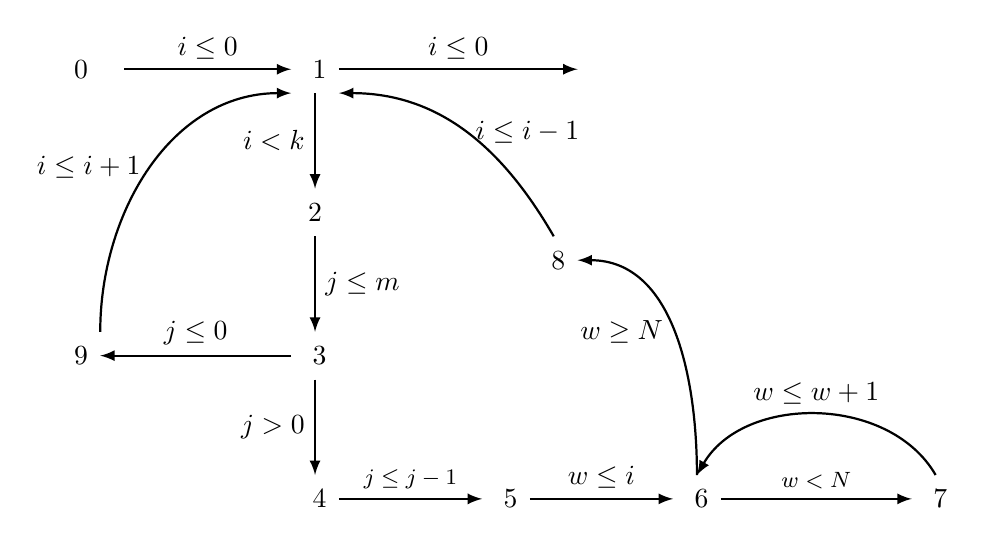
\begin{tikzpicture}[scale=\textwidth/20cm,samples=200]
                \draw[] (-5, 10) circle (0pt) node{{ $0$}};
                \draw[] (0, 10) circle (0pt) node{{ $1$}};
                \draw[] (6, 10) circle (0pt) node {{$\lex$}};
                \draw[] (0, 7) circle (0pt) node{{$2$}};
                \draw[] (0, 4) circle (0pt) node{{ $3$}};
                \draw[] (-5, 4) circle (0pt) node{{ $9$}};
                \draw[] (0, 1) circle (0pt) node{{ $4$}};
                \draw[] (4, 1) circle (0pt) node{{ $5$}};
                \draw[] (8, 1) circle (0pt) node{{ $6$}};
                \draw[] (13, 1) circle (0pt) node{{ $7$}};
                \draw[] (5, 6) circle (0pt) node{{ $8$}};
                % Counter Variables
                %
                % Control Flow Edges:
                \draw[ thick, -latex] (-4, 10)  -- node [above] {$i \leq 0$}(-0.5, 10);
                \draw[ thick, -latex] (0, 9.5)  -- node [left] {$i < k$} (0, 7.5) ;
                \draw[ thick, -latex] (0, 6.5)  -- node [right] {$j \leq m$} (0, 4.5) ;
                \draw[ thick, -latex] (0, 3.5)  -- node [left] {$j > 0$} (0, 1.5) ;
                \draw[ thick, -latex] (-0.5, 4)  -- node [above] {$j \leq 0$} (-4.5, 4) ;
                \draw[ thick, -latex] (-4.5, 4.5)  to  [out=90,in=180]  node [left] {$i \leq i + 1$ }(-0.5, 9.5);
                \draw[ thick, -latex] (0.5, 10)  -- node [above] {$i \leq 0$}  (5.5, 10);
                \draw[ thick, -latex] (0.5, 1)  -- node [above] {{\footnotesize $j \leq j - 1$}}  (3.5, 1);
                \draw[ thick, -latex] (4.5, 1)  -- node [above] {$w \leq i$}  (7.5, 1);
                \draw[ thick, -latex] (8.5, 1)  -- node [above] {{\footnotesize $w < N$}}  (12.5, 1);
                \draw[ thick, -latex] (8, 1.5)  to [out=90,in=0] node [left] {{$w \geq N$}}  (5.5, 6);
                \draw[ thick, -latex] (13, 1.5)  to  [out=120,in=60] node [above] {$w \leq w + 1$}  (8, 1.5);
                \draw[ thick, -latex] (5, 6.5)  to  [out=120,in=0]  node [right] {$i \leq i - 1$ }(0.5, 9.5);
                \end{tikzpicture}
%     \caption{}
%     \end{centering}
%     \end{subfigure}
% \begin{subfigure}{.2\textwidth}    
% \begin{centering}
    {\small
$
    \begin{array}{ll}
        \tpath_0 = (0 \to 1)
        &
        \tpath_4 = (6 \to 8 \to 3)
        \\        
        \tpath_1 = (1 \to 2 \to 3)
        &
        \tpath_5 = (3 \to 9 \to 1)
        \\
        \tpath_2 = (3 \to 4 \to 5 \to 6)
        &
        \tpath_6 = (1 \to \lex)
        \\
        \tpath_3 = (6 \to 7 \to 6)
    \end{array}
$
$
    \begin{array}{l}
        \rprog_1 = {\rprepeat(\tpath_1; 3: {\rprepeat(\tpath_2; 6 : {\rprepeat(\tpath_3)}; \tpath_4)}; \tpath_5)}
        \\
        \rprog_3 = {\rprepeat(\tpath_2; 6 : {\rprepeat(\tpath_3)}; \tpath_4)}
    \end{array}
$
}
\caption{}
\end{centering}
\end{subfigure}
    \caption{
    (a) An example of three nested loops with related iterator variables.
    (b) The abstract transition graph, simple transition paths and loop body.}
        \label{fig:threeWhile-overview}
    \end{figure}

%%%%%%%%%%%%%%%%%%%%%%%%%%%%%%%%%%%%%%%%%%%%%%%%%%%%%%%%%%%%%%%%%%%%%%%%%%%%%%%%%%%%%%%%%%%%%%%%%%%%%%%%%%%%%%%%%%%%%%%%%%%%%%%%%%%%%%%%%
%%%%%%%%%%%%%%%%%%%%%%%%%%%%%%%%%%%%%%%%%%%%%%%% The Program Model and Definition %%%%%%%%%%%%%%%%%%%%%%%%%%%%%%%%%%%%%%%%%%%%%%%%%%%%%%%%
%%%%%%%%%%%%%%%%%%%%%%%%%%%%%%%%%%%%%%%%%%%%%%%%%%%%%%%%%%%%%%%%%%%%%%%%%%%%%%%%%%%%%%%%%%%%%%%%%%%%%%%%%%%%%%%%%%%%%%%%%%%%%%%%%%%%%%%%%
\section{{Program Model}}
\label{sec:language}
\subsection{Labeled Language}
\[
\begin{array}{llll}
\mbox{Arithmetic Operators} 
& \oplus_a & ::= & + ~|~ - ~|~ \times 
%
~|~ \div ~|~ \emax ~|~ \emin
\\  
\mbox{Arithmetic Expression} 
& \aexpr & ::= & 
n ~|~ {x} ~|~ \aexpr \oplus_a \aexpr  
 ~|~ \elog \aexpr  ~|~ \esign \aexpr
\\
\mbox{Boolean Expression} & \bexpr & ::= & 
%
\etrue ~|~ \efalse  ~|~ \neg \bexpr
 ~|~ \bexpr \land \bexpr
%
~|~ \bexpr \lor \bexpr
~|~ \aexpr \leq \aexpr 
~|~ \aexpr < \aexpr 
~|~ \aexpr = \aexpr 
\\
\mbox{Expression} & \expr & ::= & v ~|~ \aexpr ~|~ \bexpr ~|~ [\expr, \dots, \expr]
\\  
%
\mbox{Value} 
& v & ::= & { n \in \mathbb{N}^{\infty} ~|~ \etrue ~|~ \efalse ~|~ [] ~|~ [v, \dots, v]} \\
%
% \\%
\mbox{Label} 
& l & \in & (\mathbb{N} \cup \{\lin, \lex\}) 
\\ 
%
\mbox{Labeled Command} 
& {c} & ::= &  
\clabel{\assign{x}{\expr}}^l 
~|~  \clabel{\eskip}^l
~|~ \ewhile \clabel{\bexpr}^{l} \edo ({c})
~|~ \eif(\clabel{\bexpr}^{l} , {c}, {c}) 
~|~ {c};{c}  
\\ 
\mbox{Event} 
& \event & ::= & 
({x}, l, v) ~ \mbox{Assignment Event} 
% \\
% &&& 
~|~(\bexpr, l, v) ~ \mbox{Testing Event}
\\
\mbox{Trace} & \trace
& ::= & [] ~|~ \trace :: \event
\\
\end{array}
\]
We denote by $\infty$ a value s.t. $n < \infty $ for all $n \in \mathbb{N}$.
We use following notations to represent the sets of corresponding terms:
\[
\begin{array}{lll}
\vardom & : & \mbox{Set of Variables}  
\\ 
%
\booldom & : & \mbox{Set of Boolean Expressions}  
\\ 
%
\cdom & : & \mbox{Set of Commands} 
\\ 
%
\eventset  & : & \mbox{Set of Events}  
\\
%
\eventset^{\asn}  & : & \mbox{Set of Assignment Events}  
\\
%
\eventset^{\test}  & : & \mbox{Set of Testing Events}  
\\
%
\ldom  & : & \mbox{Set of Labels}  
\\
%
\highlight{\ftdom} & : & \mbox{\highlight{Set of All Finite Execution Traces}}
\\
\highlight{\inftdom} & : & \mbox{\highlight{Set of Infinite  Execution Traces}}
\\
\highlight{\tdom} & : & \mbox{\highlight{Set of All Finite Or Infinite  Execution Traces}}
\\ 
%
\inpvar(c) & : & \mbox{Set of Program $c$'s Input Variables}  
\\
%
\ftdom_0(c) & : & \mbox{Set of Program $c$'s Initial Traces.}
\\ & & \mbox{Each initial trace $\trace_0 \in \ftdom_0(c)$ is finite and every input variable of the program $c$ has an initial value in $\trace_0$.}
\end{array}
\]
%
\subsection{{Trace-based Operational Semantics}}
\label{sec:operational_semantics}
\paragraph{Event}
An event is a triple.
Its first element is the variable name $x$,
or a boolean expression (from the guard of if or while command), 
following by 
 the label, $l$ associated to this command and the value assigned to the variable.

 We have two kinds of events: \emph{assignment events} and \emph{testing events},
 and we use $\eventset^{\asn}$ and $\eventset^{\test}$ to denote the set of all assignment events and testing events, respectively.

 An \emph{assignment event} tracks the execution of an assignment and consists of the assigned variable, the label of the command that generates it, the value assigned to the variable.

 A \emph{testing event} tracks the execution of if and while commands, specifically the evaluation of the boolean expression $b$ in the guard of a $\eif(\clabel{b}^l, c_1, c_2)$ command or $\ewhile \clabel{b}^l \edo c$.
 It consists of the boolean expression $b$ in the guard of the command, the label of the guard, the result of evaluating the guard.
%
\[
\begin{array}{llll}
  \mbox{Event} 
  & \event & ::= & 
  ({x}, l, v) ~ \mbox{Assignment Event} 
  ~|~(\bexpr, l, v) ~ \mbox{Testing Event}
\end{array}
\]
Event projection operators $\pi_i$ projects the $i^{th}$ element from an event: 
% \\
$\pi_i : 
\eventset \to \vardom \cup \booldom \cup \ldom $

\paragraph{Trace.}
%
A trace $\trace \in \tdom $ is a list of events, 
collecting the events generated along the program execution. 
\[
\begin{array}{llll}
\mbox{Trace} & \trace
& ::= & [] ~|~ \trace :: \event
\end{array}
\]
A trace can be regarded as the program history, 
which records all the evaluations for assignment commands and guards in $\eif$ and $\ewhile$ command.
\\
\highlight{If a program doesn't terminate when executing under some initial trace, it produces an infinite trace $\trace \in \tdom^{\infty}$.
$\tdom^{\infty}$ is the set of all finite or infinite traces.}
\\
$\tracecat: \mathcal{T} \to \mathcal{T} \to \mathcal{T}$ is the trace concatenation operator, which combines two traces,
and $\vcounter : \mathcal{T} \to \mathbb{N} \to \mathbb{N}$ is the counting operator, 
which counts the occurrence of a labeled variable in the trace. When the input trace is infinite, it returns $\infty$.
$\event \in \trace $ or $\event \notin \trace $ denotes that $\event$ belongs to $trace$ or not.
All the definition details are in the appendix.
%
The counter operator is abused when the input is a sequence of labels $L = (l_1, \cdots, l_n)$ by counting the occurrence
of this sequence in trace. Specifically,
$\vcounter(\trace :: (\_, l_1, \_) :: \cdots :: (\_, l_n, \_), L ) \triangleq \vcounter(\trace, L) + 1$
and $\vcounter(\trace :: (\_, l, \_), L ) 
\triangleq \vcounter(\trace, L) ~ l \neq l_n$, etc.
The operator $\tlabel : \tdom \to \mathcal{P}{(\ldom)}$ gives the set of labels in every event belonging to a trace.
$\tlabel{(\trace  :: (\_, l, \_)])} \triangleq \{l\} \cup \tlabel{(\trace )}$ and $\tlabel({[ ]}) \triangleq \{\}$.
%
\paragraph{Environment.} $\env : {\ftdom}  \to \vardom \to(\mathbb{N} \cup \{\bot\})$
\[
\begin{array}{llll}
\env(\trace  \traceadd (x, l, v)) x \triangleq v
&
\env(\trace \traceadd (y, l, v)) x \triangleq \env(\trace) x, y \neq x
&
\env(\trace \traceadd (b, l, v)) x \triangleq \env(\trace) x
&
\env({[]} ) x \triangleq \bot
\end{array}
\]
%
\begin{lem}[Initial Traces]
  \label{lem:initial_trace}
  \[
    \forall c \in \cdom, \trace \in \ftdom \st \trace \in \ftdom_0(c) \iff 
    \forall x \in \inpvar(c) \st \env(\trace_0) x \neq \bot
    \]
\end{lem}
%
\paragraph{Configuration.}
%
\paragraph{Expression Semantics}
The evaluation notation for arithmetic expression is $\econfig{} : \mathcal{A} \to \tdom \to \mathcal{V}$.
The $\econfig{\aexpr}(\trace)$ evaluates an arithmetic expression $\aexpr$ under trace $\trace$ following the arithmetic expression evaluation rules in Figure~\ref{fig:aexpr-eval}.
\begin{figure}
\begin{mathpar}
  \boxed{ \econfig{} \, : \, \mbox{Arithmetic Expression $\to$ Trace $\to$ Arithmetic Value}}
  \\
  \inferrule{ 
    \empty
  }{
   \econfig{n} (\trace)
   = n
  }
  \and
  \inferrule{ 
    \env(\trace) x = v
  }{
   \econfig{x} 
   = v
  }
  \and
  \inferrule{ 
    \econfig{\aexpr_1}(\trace) = v_1
    \and 
    \econfig{\aexpr_2}(\trace) = v_2
    \and 
     v_1 \oplus_a v_2 = v
  }{
   \econfig{\aexpr_1 \oplus_a \aexpr_2} 
   = v
  }
  \and
  \inferrule{ 
    \econfig{\aexpr}(\trace) = v'
    \and 
    \elog v' = v
  }{
   \econfig{\elog \aexpr}(\trace) 
   = v
  }
  \and
  \inferrule{ 
    \econfig{\aexpr}(\trace) = v'
    \and 
    \esign v' = v
  }{
   \econfig{\esign \aexpr} 
   = v
  }
   \end{mathpar}
   \caption{Evaluation Rules of Arithmetic Expression}
   \label{fig:aexpr-eval}
   \end{figure}

 The evaluation rules for boolean expression and standard expression are in Figure~\ref{fig:bexpr-eval} and Figure~\ref{fig:expr-eval}.
 \begin{figure}
  \begin{mathpar}
  \boxed{ \barrow \, : \, \mbox{ Boolean Expression $\times$ Trace $\rightarrow$ Boolean Value} }
  \\
  \inferrule{ 
    \empty
  }{
   \config{\efalse, \trace} 
   \barrow \efalse
  }
  \and 
  \inferrule{ 
    \empty
  }{
   \config{\etrue, \trace} 
   \barrow \etrue
  }
  \and 
  \inferrule{ 
    \config{\bexpr, \trace} \barrow v'
    \and 
    \neg v' = v
  }{
   \config{\neg \bexpr, \trace} 
   \barrow v
  }
  \and 
  \inferrule{ 
    \config{\bexpr, \trace_1} \barrow v_1
    \and 
    \config{\bexpr, \trace_2} \barrow v_2
    \and 
     v_1 \land v_2 = v
  }{
   \config{\bexpr, \trace_1 \land \bexpr_2} 
   \barrow v
  }
  \and 
  \inferrule{ 
    \config{\bexpr, \trace_1} \barrow v_1
    \and 
    \config{\bexpr, \trace_2} \barrow v_2
    \and 
     v_1 \lor v_2 = v
  }{
   \config{\bexpr, \trace_1 \lor \bexpr_2} 
   \barrow v
  }
  \end{mathpar}
  \caption{Evaluation Rules of Boolean Expression}
  \label{fig:bexpr-eval}
  \end{figure}
  
  \begin{figure}
    \begin{mathpar}
  \boxed{ \earrow \, : \, \mbox{Expression $\times$ Trace $\rightarrow$ Value} }
  \\
  \inferrule{ 
    \econfig{\aexpr}(\trace) = v
  }{
   \config{\aexpr, \trace} 
   \earrow v
  }
  \and
  \inferrule{ 
    \config{\bexpr, \trace} \barrow v
  }{
   \config{\bexpr, \trace} 
   \earrow v
  }
  \and
  \inferrule{ 
    \config{\expr_1, \trace} \earrow v_1
    \cdots
    \config{\expr_n, \trace} \earrow v_n
  }{
   \config{ [\expr_1, \cdots, \expr_n], \trace} 
   \earrow [v_1, \cdots, v_n]
  }
  \and
  \inferrule{ 
    \empty
  }{
   \config{v, \trace} 
   \earrow v
  }
   \end{mathpar}
   \caption{Evaluation Rules of Standard Expression}
   \label{fig:expr-eval}
   \end{figure}

\paragraph{Operational Semantics Rules}
%
The trace based operational semantics rules are defined as in Figure~\ref{fig:command-os}.
\begin{figure}
  \begin{mathpar}
\boxed{
\mbox{Command $\times$ Trace}
\xrightarrow{}
\mbox{Command $\times$ Trace}
}
\and
\boxed{\config{{c, \trace}}
\xrightarrow{} 
\config{{c',  \trace'}}
}
%
\\
%
\inferrule
{
\config{\expr, \trace} \earrow v
  \and
\event = ({x}, l, v)
}
{
\config{\clabel{\assign{{x}}{\expr}}^{l},  \trace } 
\xrightarrow{} 
\config{\clabel{\eskip}^l, \trace \traceadd \event}
}
~\rname{assn}
\and
%
\inferrule
{
  \config{\bexpr, \trace} \earrow \etrue
 \and 
 \event = (\bexpr, l, \etrue)
}
{
\config{{\ewhile \clabel{\bexpr}^{l} \edo (c), \trace}}
\xrightarrow{} 
\config{{
c; \ewhile \clabel{\bexpr}^{l} \edo (c),
\trace \traceadd \event}}
}
~\rname{while-t}
%
%
\and
%
\inferrule
{
  \config{\bexpr, \trace} \earrow \efalse
 \and 
 \event = (\bexpr, l, \efalse)
}
{
\config{{\ewhile \clabel{\bexpr}^{l} \edo (c), \trace}}
\xrightarrow{} 
\config{{
  \clabel{\eskip}^l,
\trace \traceadd \event}}
}
~\rname{while-f}
%
%
\and
%
%
\inferrule
{
\config{{c_1, \trace}}
\xrightarrow{}
\config{{c_1',  \trace'}}
}
{
\config{{c_1; c_2, \trace}} 
\xrightarrow{} 
\config{{c_1'; c_2, \trace'}}
}
~\rname{seq1}
%
\and
%
\inferrule
{
  \config{{c_2, \trace}}
  \xrightarrow{}
  \config{{c_2',  \trace'}}
}
{
\config{{\clabel{\eskip}^l; c_2, \trace}} \xrightarrow{} \config{{ c_2', \trace'}}
}
~\rname{seq2}
%
\and
%
%
\inferrule
{
  \config{\bexpr, \trace} \earrow \etrue
 \and 
 \event = (\bexpr, l, \etrue)
}
{
\config{{
\eif(\clabel{\bexpr}^{l}, c_1, c_2), 
\trace}}
\xrightarrow{} 
\config{{c_1, \trace \traceadd \event}}
}
~\rname{if-t}
%
\and
%
\inferrule
{
 \config{\bexpr, \trace} \earrow \efalse
 \and 
 \event = (\bexpr, l, \efalse)
}
{
\config{{\eif(\clabel{\bexpr}^{l}, c_1, c_2), \trace}}
\xrightarrow{} 
\config{{c_2, \trace \traceadd \event}}
}
~\rname{if-f}
%
\end{mathpar}
\caption{Operational Semantics Rules}
\label{fig:command-os}
\end{figure}


Given an initial trace $\trace_0 \in \ftdom_0(c)$ of the program $c$,
we use $\to^*$ for the reflexive and transitive closure of $\to$. 
If $\config{c, \trace_0} \rightarrow^{*} \config{\clabel{\eskip}^l, \trace_0 \tracecat \trace}$,
then the program's execution terminates and produces a finite execution trace $\trace \in \ftdom$.
\\
\begin{defn}[Non-terminating and Infinite Trace]
  \label{def:non-terminating}
  Given a program $c$ and an initial trace $\trace \in \ftdom_0(c)$,
  when $c$ executes with $\trace$,  we define the execution of $c$ under $\trace$ is non-terminating and produces an infinite trace $\trace' \in \inftdom$, as 
  $\config{c, \trace_0} \uparrow^{\infty} \trace' \in \lim(\uparrow)$
  where the limit is defined as follows.
  \[
    \begin{array}{l}
      \lim(\uparrow) 
      % \in \left( (\cdom \times \ftdom) \times (\cdom \times \inftdom) \right) 
      \triangleq 
    \\ \quad
    \Big\{
      (\config{c, \trace}, \trace') ~\vert~ 
      c\in \cdom, \trace \in \ftdom_0(c),
      \trace' \in \inftdom 
      \land \exists \trace_0 \in \ftdom, c_0 \in \cdom \st 
      \config{c, \trace} \to \config{c_0, \trace_0}
      \\ \qquad \qquad \qquad 
      \land \forall i \in \mathbb{N}, \exists \trace_i, \trace_{i + 1} \in \ftdom, \trace'' \in \inftdom, c_i, c_{i + 1} \in \cdom \st 
      \config{c_i, \trace_i} \to \config{c_{i + 1}, \trace_{i + 1}} 
      \land  \trace' = \trace_{i + 1} \tracecat \trace''
    \Big\}
    \end{array}
  \]
\end{defn}
%
% \begin{defn}[Non-terminating and Infinite Trace (alternative way)]
%   \label{def:non-terminating-2}
%   Given a program $c$ and an initial trace $\trace_0 \in \ftdom_0(c)$,
%   when $c$ executes with $\trace_0$,  we define $c$ is non-terminating under $\trace_0$, $\config{c, \trace_0} \uparrow^{\infty}$ if and only if there exists a function
%   $f : \mathbb{N} \to \cdom \times \tdom$ such that $f(0) = \config{c, \trace_0}$ and
%   for every $i \in \mathbb{N}$ there exist  $\trace_i, \trace_{i + 1}\in \tdom$, $c_i, c_{i + 1} \in \cdom$ such that  $f(i) = \config{c_i, \trace_i}$, $f(i + 1) =  \config{c_{i + 1}, \trace_{i + 1}}$ and
%   $\config{c_i, \trace_i} \to \config{c_{i + 1}, \trace_{i + 1}}$. 
%   \[
%     \begin{array}{l}
%     \forall \trace_0 \in \ftdom_0(c), c \in \cdom \st
%     \config{c, \trace_0} \uparrow^{\infty}
%     \\
%     \iff \exists f : \mathbb{N} \to \cdom \times \tdom \st 
%     f(0) = \config{c, \trace_0}
%     \\ \qquad \land
%     \forall i \in \mathbb{N}, \exists \trace_i, \trace_{i + 1} \in \tdom, c_i, c_{i + 1} \in \cdom\st 
%     \\ \qquad \quad
%     f(i) = \config{c_i, \trace_i}$, $f(i + 1) =  \config{c_{i + 1}, \trace_{i + 1}} \land \config{c_i, \trace_i} \to \config{c_{i + 1}, \trace_{i + 1}}
%     \end{array}
%   \]
%   Given a program $c$ and an initial trace $\trace_0 \in \ftdom_0(c)$, if $\config{c, \trace_0} \uparrow^{\infty}$, 
%   let $f$ be the function such that for every $i \in \mathbb{N}$,  $\trace_i, \trace_{i + 1}\in \tdom$, $c_i, c_{i + 1} \in \cdom$ where $\config{c_i, \trace_i} \to \config{c_{i + 1}, \trace_{i + 1}}$, we have $f(i) = \config{c_i, \trace_i}$, $f(i + 1) =  \config{c_{i + 1}, \trace_{i + 1}}$. 
%   Let $\pi_2 : (\cdom \times \tdom) \to \tdom$ be the projector which projects the trace from a configuration,
%   then we define $\config{c, \trace_0} \uparrow^{\infty} \trace'$ produces an infinite trace $\trace' = \pi_2(\lim\limits_{i \to \infty}(f(i))) \in \inftdom$.
%   \[ \trace' = \lim( \pi_2 \circ (f(i))). \]
% \end{defn}
% %

% \begin{defn}[Non-terminating and Infinite Trace (third way)]
%   \label{def:infinite-trace}
%   Given a program $c$ and an initial trace $\trace_0 \in \ftdom_0(c)$,
%   when $c$ executes with $\trace_0$,  we define $c$ is non-terminating under $\trace_0$, denoted as $\config{c, \trace_0} \uparrow^{\infty} \trace'$ and produce an infinite trace $\trace' \in \inftdom$ 
%   if and only if there exists a function
%   $f : \mathbb{N} \to \cdom \times \tdom$ such that $f(0) = \config{c, \trace_0}$ and
%   for every $i \in \mathbb{N}$ there exist  $\trace_i, \trace_{i + 1}\in \tdom$, $c_i, c_{i + 1} \in \cdom$ such that  $f(i) = \config{c_i, \trace_i}$, $f(i + 1) =  \config{c_{i + 1}, \trace_{i + 1}}$ and
%   $\config{c_i, \trace_i} \to \config{c_{i + 1}, \trace_{i + 1}}$. 
%   \[
%     \begin{array}{l}
%     \forall \trace_0 \in \ftdom_0(c), \trace' \in \inftdom, c \in \cdom \st
%     \config{c, \trace_0} \uparrow^{\infty} \trace'
%     \\
%     \iff \exists f : \mathbb{N} \to \cdom \times \tdom \st 
%     f(0) = \config{c, \trace_0}
%     \\ \qquad \land
%     \forall i \in \mathbb{N}, \exists \trace_i, \trace_{i + 1} \in \tdom, c_i, c_{i + 1} \in \cdom\st 
%     \\ \qquad \quad
%     f(i) = \config{c_i, \trace_i}$, $f(i + 1) =  \config{c_{i + 1}, \trace_{i + 1}} \land \config{c_i, \trace_i} \to \config{c_{i + 1}, \trace_{i + 1}}.
%     \end{array}
%   \]
%   Let $\pi_2 : (\cdom \times \tdom) \to \tdom$ be the projector which projects the trace from a configuration,
%   then the infinite trace $\trace'$ produced by $\config{c, \trace_0} \uparrow^{\infty} \trace'$ is
%   \[ \trace' = \pi_2(\lim\limits_{i \to \infty}(f(i))) \in \inftdom. \]
% \end{defn}
%
This follows the maximal trace semantics in \cite{cousot2019abstract} Section 2.5 Equation (12).
\\
If we observe the operational semantics rules, we can find that no rule will shrink the trace. 
So we have the Lemma~\ref{lem:tracenondec} with proof in Appendix~\ref{apdx:lem_language}, 
specifically the trace has the property that its length never decreases during the program execution.
\begin{lem}
  [Trace Non-Decreasing]
  \label{lem:tracenondec}
  For any program $c \in \cdom$ and initial trace $\trace_0 \in \ftdom_0(c)$,
  if there exists $\trace \in \tdom$ and $c' \in \cdom $ such that $\config{c, \trace_0} \rightarrow^{*} \config{c', \trace} $ or 
  $\config{c, \trace_0} \uparrow^{\infty} \trace$  
  then there exists a trace $\trace' \in \tdom$ such that $\trace_0 \tracecat \trace' = \trace$ formally as follows.
  %
  \[
    \begin{array}{l}
    \forall \trace_0 \in \ftdom_0(c), \trace \in \tdom, c, c' \in \cdom \st
    \Big( \config{c, \trace_0} \rightarrow^{*} \config{c', \trace} 
    \lor  \config{c, \trace_0} \uparrow^{\infty} \trace \Big)
    \\ \quad
    \implies \exists \trace' \in \tdom \st \trace_0 \tracecat \trace' = \trace 
    \end{array}
    \]
  \end{lem}
  % \begin{lem}
  %   [Trace Non-Decreasing (based on the alternative non-termination definition)]
  %   \label{lem:tracenondec2}
  %   For any program $c \in \cdom$ and initial trace $\trace_0 \in \ftdom_0(c)$,
  %   \begin{itemize}
  %     \item if there exists $\trace \in \tdom$ and $c' \in \cdom $ such that $\config{c, \trace_0} \rightarrow^{*} \config{c', \trace} $
  %     then there exists a trace $\trace' \in \ftdom$ such that $\trace_0 \tracecat \trace' = \trace$;
  %     \item if $\config{c, \trace_0} \uparrow^{\infty} $ and produces an infinite trace $\trace \in \inftdom$ as defined in Definition~\ref{def:non-terminating}
  %     then there exists an infinite trace $\trace' \in \inftdom$ such that $\trace_0 \tracecat \trace' = \trace$ formally as follows.  
  %   \end{itemize}
  %   %
  %   \[
  %     \begin{array}{l}
  %     \forall \trace_0 \in \ftdom_0(c), \trace \in \tdom, c, c' \in \cdom \st
  %     \config{c, \trace_0} \rightarrow^{*} \config{c', \trace} 
  %     \implies \exists \trace' \in \ftdom \st \trace_0 \tracecat \trace' = \trace 
  %     \\
  %     \todomath{\land \config{c, \trace_0} \uparrow^{\infty} \implies \exists \trace' \in \inftdom \st \trace_0 \tracecat \trace' \in \inftdom}
  %     \end{array}
  %     \]
  %   \end{lem}
\section{{Reachability Bound}}
\label{sec:rb-def}
The operator $\lvar: \cdom \to \mathcal{P}(\ldom)$,
computes the set of labels
% assigned variables and labeles variables 
for a labeled command $c$ defined as follows,
% \begin{defn}[Program Labels
% ($\lvar : \cdom \to \mathcal{P}(\ldom)$]
% \label{def:lvar}
% {\small
% $$
%   \lvar(c) \triangleq
%   \left\{
%   \begin{array}{ll}
%       \{l\}                  
%       & {c} = [{\assign x e}]^{l} 
%       \\
%       \lvar({c_1}) \cup \lvar({{c_2}})  \cup \{l\} 
%       & {c} = {c_1};{c_2}
%       \\
%       \lvar(c_1) \cup \lvar({{c_2}}) \cup \{l\} 
%       & {c} =\eif([\bexpr]^{l}, c_1, c_2) 
%       \\
%       \lvar({{c}'}) \cup \{l\} 
%       & {c}   = \ewhile ([\bexpr]^{l}, {c}')
% \end{array}
% \right.
% $$
% }
% \end{defn}
%
Every label and every labeled command in a program is unique, formally as follows with proof in Appendix~\ref{apdx:lemma_sec123}.
\begin{lem}[Uniqueness of the Program Labels]
  \label{lem:label_unique}
  For every program $c \in \cdom$ and every two labels such that
  $i, j \in \lvar(c)$, then $i \neq j$.
  \[
    \forall c \in \cdom, i, j \in \ldom \st i, j \in \lvar(c)\implies i \neq j.
    \]
\end{lem}
%
The free variables
showing up in $c$, which aren't defined before be used, are actually the input variables of this program.
%
\begin{defn}[Reachability-Bound]
  \label{def:rb}
  For a program ${c}$ and a location $l \in \lvar(c)$ in this program,
% its 
% $\exeRB({c}, l)$ 
a function $f(c, l) : \tdom_0(c) \to (\mathbb{N} \cup \{\infty\})$ is a \emph{Reachability-Bound} for $l$ if and only if
\highlight{
\[
  \forall \trace_0 \in \tdom_0(c), \trace \in \tdominf \st 
  \Big(
    \config{{c}, \trace_0} \to^{*} \config{\eskip, \trace_0 \tracecat \vtrace} 
    \lor 
    \config{{c}, \trace_0} \to^{\infty} \config{\cdot, \trace_0 \tracecat \vtrace} 
  \Big)
  \implies f({c}, l)(\trace_0) \geq \vcounter(\vtrace, l) 
  \]
}
\end{defn}
\highlight{
Given a program point $l$ in $c$, our algorithm (defined below) computes a Reachability-Bound for it.
It is easy to compute a trivial \emph{Reachability-Bound} $f(c, l): \tdom_0(c) \to \infty$, but it is not interesting to us.
\\
In the following sections, we only focus on computing a finite \emph{reachability-bound} for program's given location and considering the executions that terminates.
Ideally, we aim to compute a precise reachability-bound as follows.
}
\begin{defn}[Precise Reachability-Bound]
  \label{def:exe_rb}
  For a program ${c}$ and a location $l \in \lvar(c)$ in this program,
% its 
$\exeRB({c}, l): \tdom_0(c) \to (\mathbb{N} \cup \{\infty\})$ is a \emph{Precise Reachability-Bound}  if and only if,
%  satisfying
%  defined as follows,
% over all possible traces,
%
\highlight{
\[
  \forall \trace_0 \in \tdom_0(c), \trace \in \tdom \st 
  \Big(
    \config{{c}, \trace_0} \to^{*} \config{\eskip, \trace_0 \tracecat \vtrace} 
    \lor 
    \config{{c}, \trace_0} \to^{\infty} \config{\cdot, \trace_0 \tracecat \vtrace} 
  \Big)
  \implies \exeRB({c}, l)(\trace_0) = \vcounter(\vtrace, l) 
  \]
}
\end{defn}

%%%%%%%%%%%%%%%%%%%%%%%%%%%%%%%%%%%%%%%%%%%%%%%%%%%%%%%%%%%%%%%%%%%%%%%%%%%%%%%%%%%%%%%%%%%%%%%%%%%%%%%%%%%%%%%%%%%%%%%%%%%%%%%%%%%%%%%%%
%%%%%%%%%%%%%%%%%%%%%%%%%%%%%%%%%%%%%%%%%%%%%%%% The Reachability Bound Algorithm %%%%%%%%%%%%%%%%%%%%%%%%%%%%%%%%%%%%%%%%%%%%%%%%%%%%%%%%
%%%%%%%%%%%%%%%%%%%%%%%%%%%%%%%%%%%%%%%%%%%%%%%%%%%%%%%%%%%%%%%%%%%%%%%%%%%%%%%%%%%%%%%%%%%%%%%%%%%%%%%%%%%%%%%%%%%%%%%%%%%%%%%%%%%%%%%%%
\section{Path Sensitive Reachability Bound Analysis}
\label{sec:psrb-alg}
In this section, we present our static program analysis algorithm for computing 
% an upper bound on the 
% execution-based reachability times 
the \emph{reachability-bound} for every program point $l$ in a program $c$ in a path sensitive manner.
% , as defined in last section.
%
% In order to have the upper bound of the reachability for every label of a program $c$, we design 
% a path sensitive reachability bound analysis algorithm {\THESYSTEM}.
The algorithm is summarized into the following steps,
% \begin{figure}
%   \centering    
% \includegraphics[width=1.0\columnwidth]{adapfun.png}
%   \vspace{-0.3cm}
%   \caption{The overview of {\THESYSTEM}}
%   \label{fig:adaptfun}
%   \vspace{-0.5cm}
% \end{figure}
%
\\
% \framebox{
    % \text{
    1. Compute Abstract Transition graph, $\absG(c)$ through program abstraction.
    % }
    \\
    % \text{
    2. Compute refined program by \cite{GulwaniJK09}. $\rprog = API(\absG(c))$
    \\
    3. Compute local bound $\outinB(\tpath, c)$
    \\
    4. Compute Reachability-Bound $\psRB = \inoutB(\tpath, c)$
    % }
% }
%
\begin{enumerate}
\item  In Section~\ref{sec:progabs}, we first construct an abstract transition graph based on $c$, by computing an abstract transition 
for every labeled command. 
This graph is used in the following sections
%  from Section~\ref{sec:refine} to Section~\ref{sec:psrbcompute} 
for computing the path-sensitive reachability-bound of a program location.
% see Section~\ref{sec:alg_vertexgen}
\item The second step in Section~\ref{sec:refine}
refines the multiple-paths loops in the program
% this program path sensitively, 
based on the abstract transition graph.
This step transforms the multiple-paths loops into multiple loops where
the interleaving of paths is explicit.
% \item Section~\ref{sec:lbcompute} computes the ranking function  
% \footnote{\textbf{ranking function} is the named used in \cite{SinnZV14}
% and \textbf{local bound} is the name used in \cite{ZulegerGSV11}, \cite{sinn2017complexity}.
% We refer to the two names as the same meaning in this paper.} for each edge in a program's abstract transition graph,
% and estimates the upper bounds on every ranking function's maximum value and every edge's execution times path-insensitively.
% path-insensitive reachability upper bound for every while loop command in $c$.
\item Section~\ref{sec:outinalg} performs the \textbf{Outside-In} algorithm and computes
the upper bound for the execution times for every path in a refined loop locally.
It first computes the ranking function  
\footnote{\textbf{ranking function} is the named used in \cite{SinnZV14}
and \textbf{local bound} is the name used in \cite{ZulegerGSV11}, \cite{sinn2017complexity}.
We refer to the two names as the same meaning in this paper.} 
for each edge in a program's abstract transition graph,
and estimates the upper bounds on every ranking function's maximum value and every path's execution times.
% , named \textbf{Outside-In} bound.
% path-sensitive local bounds.
\item Section~\ref{sec:inoutalg}
performs the \textbf{Inside-Out} algorithm and 
computes the path-sensitive reachability-bound for every program point,
It first computes the upper bound for the execution times of
every simple path in the refined program globally. 
Then it sums up the bounds of paths contains certain program point as its path-sensitive reachability-bound.
%  named \textbf{Inside-Out} bound.
% abstract transition graph.
% \item Section~\ref{sec:psrbcompute} computes the path-sensitive reachability-bound for every program point
% %  in this program 
% based on the above results.
%  by
%  ?summarizing 
% the path-sensitive reachabilitybound of each edge on the abstract transition graph.
% \item The Section~\ref{sec:reachabilitybound_algorithm} computes program's reachability bound in two steps as follows.
\end{enumerate}
% \subsection{Constraint Program}
\label{sec:abs_prog}
% \textbf{Step 1: Program Abstract Execution Control Flow Graph}
The Constraint program is an Abstract Transition Graph,
% For a program $c$, this analysis first generates its abstract execution control flow graph notated as follows,
\[\absG(c) =(\absV(c), \absE(c)).\]
%
$\absV(c)$ is the set of program $c$'s control location, each edge in $\absE(c)$ is a transition
between two control locations if and only if there is a feasible control flow between the two locations.
Each edge is annotated by a constraint
from the set $\dcdom^{\top}$.
% (denoted by $\dcdom^{\top}$).
\\
\textbf{Components:} 
\\
The Vertices Set $\absV(c) = \lvar(c)\cup\{{\lex}\}$, is the set of program $c$'s control locations.
%  $\absV(c) = \lvar(c)\cup\{{\lex}\}$
\\
An edge $(l_1, dc, l_2) \in \ldom \times \dcdom^{\top} \times \ldom$, represents control flow from $l_1$ to $L_2$.
% such that control flow from $l_1$ to $l_2$.
\\
An annotation is a constraint from $\dcdom^{\top}$: Difference Constraints $\cup$ Boolean Expressions $\booldom$ $\cup \top$ represents the infinity.
\\
A difference constraint $dc: \dcdom^{\top}$,
% Difference Constraints $\cup$ Boolean Expressions $\booldom$ $\cup \top$ represents the infinity.
describes the size changes of all the program variables by executing commands from location $l_1$ to $l_2$.
\\
\textbf{Computation Steps:} 
\\
Step1: generating control flow edges $(l_1, \_, l_2)$ for all the locations $l_1, l_2 \in \lvar(c)$.
\\
Step2: computing annotation $dc$ for each edge $(l_1, \_, l_2)$.
\\
Input the commands from location $l_1$ to $l_2$.
\\
Output: a set of $\dcdom^{\top}$.
\\
% Constraint Event: 1 edge of the Constraint Program, and 
% \\
% Constraint Execution Trace : the edge set of the Constraint Program.
\textbf{Theorem Guarantee:}
Soundness and Uniqueness.
\subsection{Constraint Program Refinement}
\label{sec:refine}
Algorithm Steps:
\\
\textbf{Step1: Simple Transition Path}.
\\
% Computes the Simple Transition Paths from Constraint Program,  
% 
Simple Transition Path: $\tpath \in \paths(\absG(c))$.
\\
% For a constraint program $\absG(c)$,
A \emph{simple transition path} is a path of a constraint program, $\tpath \in \paths(\absG(c))$.
It either
\begin{itemize}
  \item contains only one loop (without any nested loop) starting from a loop header at location $l$ and go back to the same $l$;
  \item or doesn't contain a loop, starting from a loop header $l$ (or the program entrance $l_0$)
and ending with different loop header $l'$ (or the program exist $\lex$).
\end{itemize}
%
\textbf{Step2: Repeat Pattern}.
% \\
% A \emph{Repeat Pattern} ($\rprog \in \mathcal{P}({\absG(c)})$) is either a simple path or sequence of repeat patterns of this program $c$. 
% \[
%   \rpattern := \tpath ~|~ \rprepeat(\rpattern) ~|~ \rpattern; \rpattern
% \]
% Every $\rprog'$ with the annotation $\rprepeat$, (for example, $\rpattern = \rprepeat(\rpattern')$)
% can consecutively execute at least twice.
% Every two sub-repeat patterns following each other in a $\rprog$ can execute in sequence, for example in $\rpattern = \rpattern_1; \rpattern_2$,
% $\rpattern_2$ can execute after $\rpattern_1$.
% Every sub-repeat patterns in the sequence are distinct.
%  \\
% Through Path-Sensitive Refinement / Contextualization algorithm in \cite{GulwaniJK09, ZulegerGSV11},
% this step computes the repeat patterns over all \emph{simple transition path}s.
% \\
\begin{defn}[Repeat Pattern of A Program]
  \label{def:repeat-pattern}
  Given a constraint program $\absG(c)$,
  $\rpattern(c)$ is a \emph{Repeat Pattern} of $\absG(c)$ if and only if, it is a simple path or
  a sequence of \emph{repeat pattern}
  has the following syntax
  \[
    \rpattern := \tpath ~|~ \rprepeat(\rpattern) ~|~ \rpattern; \rpattern
  \] 
  and satisfying,
  \begin{itemize}
  \item every sub-repeat pattern $\rpattern' \in \rpattern(c)$ with the annotation $\rpattern$
  can consecutively execute twice
  %  when executing this program $c$ 
  w.r.t. some initial trace,
  \item every sub-repeat patter in a sequence is distinct, i.e., $\rpattern(c) = \rpattern_1; \cdots; \rpattern_n$ and 
  % $\rpattern_i, \rpattern_j \in \rpattern_1; \cdots; \rpattern_n$, 
  $\rpattern_i \neq \rpattern_j$ for every $i, j = 1, \cdots, n$,
  \item and every two continuous sub-repeat patters in a sequence can execute after each other w.r.t some initial trace,
  i.e., $\rpattern(c) = \rpattern_1; \cdots; \rpattern_n$ and for every $i = 1, \cdots, n$,
  $\rpattern_i$ can execute after $\rpattern_{i - 1}$ under some initial trace.
  \end{itemize}
\end{defn}
%
\textbf{Step3: Refined Program}.
% \\
\begin{defn}[Refined Program of A Program]
  Given a constraint program $\absG(c)$,
  its \emph{Refined Program} is either a repeat pattern, or a set of refined program, or sequence of refined program has
  the following syntax,
  \[
    \rprog :=  \rprepeat ~|~ \rpchoose\left\{\rprog\right\} ~|~ \rprog; \rprog.
  \]
  It satisfies that for every sub refined program $\rprog' \in \rprog$
  % $\rprog = \rprog_1, \cdots; \rprog_n$ and
  % $\rprog_i = \{\rpattern_{0}; \cdots; \rpattern_{i_n}\}$, $n, i_n \in \mathbb{N}$ and
  \begin{itemize}
  \item if
   $\rprog' = \rpchoose\left\{\rprog_1, \cdots, \rprog_m \right\}$,
   then all the $\rprog_1, \cdots, \rprog_m$ have the same starting and ending label,
  \item if $\rprog' = \rprog_1; \rprog_2$, then
  % and for every $\rpattern_1 \in \rprog_i$ and $\rpattern_2 \in \rprog_{i + 1}$,
  $\rprog_1$'s ending label is the same label as $\rprog_2$'s starting label.
  \end{itemize}
\end{defn}
%
%  annotation for two branches of $\eif$.
% them into
%  of this loop header
%s
\textbf{Theorem Guarantee.}
Soundness of the refinement.
\subsection{Ranking / Local Bound Computation}
\label{sec:ranking}
Steps:
\\
\textbf{Step1: Variable Constraint Collection:}
Identify the abstract events where each variable is increased, decreased and reset:
\\
$\inc: \mathcal{VAR} \to \mathcal{P}(\absE(c)) $
the set of the abstract events where the variable increase.
\\
$\inc(x) = \{(e, c) | e = (l, x' \leq x + c, l') \land e \in \absE(c)\}$
\\
$\reset: \mathcal{VAR} \to \mathcal{P}(\absE(c)) $
The set of the abstract events where the variable is reset.
\\
$\dec: \mathcal{VAR} \to \mathcal{P}(\absE(c)) $
The set of abstract events where the variable decrease.
\\
\textbf{{Step2: Assign Ranks / Local Bound to Edges}}
$\locbound: \absE(c) \to \mathcal{VAR} \cup \constdom$.
 \\
\textbf{Step3: Ranks / Local Bounds Estimation}
Estimating the bounds on the (ranks'/ local bounds') maximum value.
% , the 
\\ 
$ \varinvar: \mathcal{VAR} \cup \constdom \to \mathcal{A}_{\lin}$
% \\
% $\absclr: \absE(c) \to \mathcal{A}_{\lin}$
\\
$Incr(x) \triangleq \sum\limits_{(e, c) \in \inc(x)}\{\absclr(\absevent) \times v\}$
\\
Then estimate the bounds on the iteration times
% of the ranks / local bounds 
for each edge in a path-insensitive fashion.
% \\
% computing the loop bound in a path-insensitive way as the base step.
% \\ 
% $ \varinvar: \mathcal{VAR} \cup \constdom \to \mathcal{A}_{\lin}$
\\
$\absclr: \absevent \to \mathcal{A}_{\lin}$
\\
\textbf{Theorem Guarantee.}
Soundness of the Path-Insensitive Local Bound / Rank Estimation.
%  Require Variable Bound Computation.
\subsection{Outside-In Algorithm}
\label{sec:outinalg}
For the refined program $\rprog \in \mathcal{RP}$, the \textbf{Outside-In Algorithm} ($\outinB: \rprog \to \mathcal{A}_{in}$)
computes the \emph{OutIn} bound on the iteration numbers of every repeat pattern in this program.
\\
It is called \emph{OutIn} bound because for a repeat pattern $\rpattern$ nested
in another repeat pattern $\rpattern' = \rprepeat(\rpattern)$,
this value only bounds the iteration number of $\rpattern$ inside $\rpattern'$ by assuming $\rpattern'$ executes once.

\highlight{\textbf{Notations / Operators:}}
\\
The \emph{State}: 
$\absstate \in \mathcal{P}(\dcdom^{\top})$ : conjunctions of the edge annotations.
%  constraints.
\\
For a refined program ($\rprog$), there are the 
\\
\emph{Initial State} ($\rfinit(\rprog)$), 
\emph{Final State} ($\rffinal(\rprog)$), and \emph{Next State} ($\rfnext(\rprog)$)  $\in \absstate$.
% The \emph{Initial State}: $\rfinit : \rprog \to \absstate $.
\\
The \emph{Variable Grade Decedent}: $\varGD : \rprog \to \mathcal{A}_{in}$, is the set of the variables' variation in one iteration;
% The \emph{Initial State}: $\rfinit : \rprog \to \absstate $.

\highlight{\textbf{Omitted Computations:}}
\\
Computing the $\outinB$ bound for a refined program $\rprog$. 
\\
$\outinB(\rpchoose\{\rprog_i\}) =  \max\{\outinB(\rprog_i)\}$
\\
$\outinB(\rprepeat\{\rprog\}) =  \frac{\rfinit(\rprog) - \rffinal(\rprog)}{\varGD(\rprog)}$
\\
$\outinB(\rpseq(\rprog_1, \rprog_2)) =  \outinB(\rprog_1)+ \outinB( \rprog_2)$
\\
$\outinB(\tpath) =  1$.
\\
The computations of the operations: $\rfinit(\rprog)$,
$\rffinal(\rprog)$ $\rfnext(\tpath)$ and $\varGD : \rprog \to \mathcal{A}_{in}$ is in Appendix.
Equivalent result can be computed for $\outinB(\rprepeat\{\rprog\})$ by alternative computation method from paper \cite{GulwaniJK09} while in-efficiently.
\subsection{Inside-Out Algorithm}
\label{sec:inoutalg}
For the refined program $\rprog \in \mathcal{RP}$, the \textbf{Inside-Out Algorithm}
computes the reachability-bound on the execution numbers for every simple transition path $\tpath$ in this program $\rprog$,
through the following steps.
%
\begin{enumerate}
  \item \emph{Repeat Chain Bound:} $\rpchB(l, \tpath, \rprog) \in \mathcal{A}_{in}$.
  \\
  For every transition path $\tpath$ in a refined program $\rprog$,
  its \emph{Repeat Chain Bound} is the
  bound on its execution numbers inside its closet while loop.

  \highlight{\textbf{Omitted Computations:}}
\begin{defn}[Repeat Chain]
  \label{def:repeatchain}
For a refined program $\rprog$ and a simple transition path $\tpath$,
a \emph{Repeat Chain} $\rpch(l, \tpath, \rprog)$
is a list of repeat patterns nested in a repeat pattern with loop header annotation $l$,
%  efined program contained inside the same while loop $L$ as the $\tpath$. 
% It is computed as follows,
  % $\rpch(L_l, \tpath) \in \mathcal{P}(\rprog)$\\
\[
 \rprog_n \to \rprog_{n-1} \to \cdots \to \tpath
\]
It satisfies
 $\rprog_{i}= l : \rprepeat(\cdots, \rprog_{i - 1}, \cdots)$ and
 there isn't any nested loop header ($l'$) or $\rprepeat$ annotation between $\rprog_{i}$ and $\rprog_{i - 1}$
 for every $i = n, \cdots, 1$.
\end{defn}
%
\textbf{Repeat Chain Set}
\begin{defn}[Repeat Chain Set]
  \label{def:repeatchainset}
  For a refined program $\rprog$ and a simple transition path $\tpath$, the \emph{Repeat China Set}
  $\rpchset(l, \tpath, \rprog)$ is the set of 
  all repeat chains for $\rprog$ and $\tpath$,
  \[
    \left\{\rpch(l, \tpath, \rprog) \right\}.
 \]
\end{defn}
\textbf{Repeat Chain Bound}
\\
For every transition path $\tpath$
in its closet enclosed while loop $l$,
% $rpRB: \tpath \to \mathcal{A}_{in}$, $chsRB: (\rprog \times \tpath) \to \mathcal{A}_{in}$
% \\
% For each transition path $\tpath \in \rprog$,
% \\
% 1. First compute the path sensitive reachability choosing bound through their choose chain:
% \\
% $chsRB(\rprog_n, \tpath) = \prod\limits_{\rprog_i \in lpchain(\rprog_n, \tpath)}
% \frac{chsInit(\rprog_i, \tpath) - chsFinal(\rprog_i, \tpath)}{\varGD(\rprog_i, \tpath)}$
  \\
  $
  \begin{array}{l}
    \rpchB(l, \tpath,  \rprog) = \\
    \max \left\{ \prod\limits_{\rprog_i \in ch}  \outinB(\rprog_i) 
  ~\middle\vert~ ch \in \rpchset(l, \tpath, \rprog) \right\}
  \end{array}
  $
  \\
  \item \emph{Relative Loop Bound:} $\lpchB(l, \tpath, \rprog) \in \mathcal{A}_{\lin}$.
  \\
  For every simple transition path $\tpath$
and a loop header at location $l$ in a refined program $\rprog$,
the \emph{Relative Loop Bound} $\lpchB(l, \tpath, \rprog) \in \mathcal{A}_{\lin}$ is a symbolic expression in $\mathcal{A}_{\lin}$.
\\
This expression is a sound bound on the iteration numbers of loop $l$ relative to the simple transition path $\tpath$.
This $\tpath$'s closest enclosing loop has the loop header at $l'$ and $l'$ is nested inside the loop $l$.
\\
It estimates the iteration numbers of loop $l$ such that during these iterations, the nested loop $l'$ is executed.

%  will 
\highlight{\textbf{Omitted Computations:}}
\\
\textbf{Loop Chain}.  $\lpch(\tpath, \rprog) \in \mathcal{P}(\rprog)$.
\begin{defn}[Loop Chain]
  \label{def:loopchain}
For a refined program $\rprog$ and a simple transition path $\tpath$ in this program, the loop chain $\lpch(\tpath, \rprog)$
is
%
\[ 
\rprog_n \to \rprog_{n-1} \to \cdots \to \tpath
\]
% such that there is at least a $\rpchoose$ and isn't consecutive repeats $\rprepeat$ (i.e., at most one 
% $\rprepeat$) between any $\rprog_{i - 1}$ and $\rprog_{i}$ for $i = n, \cdots, 1$.
such that 
$\rprog_{i}= l_i : (\cdots, l_{i - 1} : \rprog_{i-1}, \cdots)$ and
 there isn't any nested loop annotation (i.e., $l'$) between $\rprog_{i}$ and $\rprog_{i - 1}$ for $i = n, \cdots, 1$.
\end{defn}
%
\highlight{
\textbf{Relative Loop Bound:}
% $\lpchB(l, \tpath, \rprog) \in \mathcal{A}_{\lin}$.
\begin{defn}[Relative Loop Bound]
  \label{def:relatedloop_bound}
For every simple transition path in a refined program $\tpath \in \rprog$
and every loop $l \in \lpch(\tpath, \rprog)$,
% where $\lpch(\tpath)  \in \rpchset(\tpath)$, 
the \emph{Relative Loop Bound} $\lpchB(l, \tpath, \rprog)$ is computed as follows,
\[
  \left\{
  \begin{array}{l}
    \rpchB(l, \tpath, \rprog)  
    \\ \qquad \rpchB(l, \tpath) \neq \bot
    \\
    \frac{\lpinit(l, \tpath) - \rffinal(\tpath)}{\lpinit(l, \tpath) - \lpnext(l, \tpath)}
     \qquad o.w.
  \end{array}
  \right\}
  \]
\end{defn}
}
The computations of the operations $\lpinit(L_i, \tpath)$ and $\lpnext(L_i, \tpath)$ are in Appendix.
%
\item The \emph{Inside-Out Bound} ($\inoutB(\tpath, \rprog) \in \mathcal{A}_{in}$).
\\
For every simple transition path $\tpath \in \rprog$,
its \emph{Inside-Out Loop Bound}
 $\inoutB(\tpath, \rprog) \in \mathcal{A}_{in}$ is 
% Compute 
the path sensitive reachability-bound on $\tpath$'s execution numbers.

\highlight{\textbf{Omitted Computations:}}
\begin{defn}[{Inside-Out Loop Bound}]
  \label{def:outin_bound}
  Given a refined program $\rprog$, for every transition path $\tpath \in \rprog$, 
  its \emph{Inside-Out Loop Bound}
  $\inoutB(\tpath, \rprog)$ is 
 % Compute 
\[
  \prod\limits_{L \in \lpch(\tpath, \rprog)} \rpchB(l, \tpath, \rprog).
% lpRB(\rprog_i, \tpath) 
% ~ \middle\vert~ l \in lp\mathcal{C}(\tpath) \right
\]
\end{defn}
% For $chain \in rpchain(\tpath)$:
% where $lpchains(\tpath)$ is set of $lpchains(\tpath)$ containing all the loop chains of $\tpath$.
\end{enumerate}
\subsection{Path Sensitive Reachability Bound Computation}

For every program control location $l \in \lvar(c)$, with $\rprog$ as its refined program,
%  in a program $c$,
its path-sensitive reachability-bound ($\psRB(l, \rprog)$) is a symbolic sound bound on the executing times of $l$.

\highlight{\textbf{Omitted Computations:}}
 \begin{defn}
  \label{def:label_psrb}
Given a program $c$ with its refined program $\rprog \in \mathcal{RP}$
%  with 
% \emph{Global Loop Bound} $\inoutB(\tpath)$
% computed for its every transition path $\tpath \in \rprog$  notated by $\inoutB(\tpath)$,
%  for each of its transition path $\tpath \in \rprog$ 
% with the \emph{Global Loop Bound}
% computed as above, notated by $\inoutB(\tpath)$.
the $\psRB(c, l)$ for every label $l \in \lvar(c)$ is computed as follows,
\\
\[ \psRB(c, l) = \sum\limits_{\tpath \in \rprog \land 
l \in \tpath} \inoutB(\tpath)\]
 \end{defn}
\begin{thm}[Soundness of the Path Sensitive Reachability Bound Estimation]
  \label{thm:pathsensitive_rb_soundness}
Given a program ${c}$, for every label $l$ of this program $c$ such that $(l, w) \in \exeRB(c)$, 
and any initial trace $\trace_0 \in \mathcal{T}_0(c)$ with 
% $\config{{c}, \trace_0} \to^{*} \config{\eskip, \trace_0\tracecat \vtrace} $ 
and $\config{\psRB(c, l), \trace_0} \earrow v$,
% for some generated evaluation trace $\vtrace \in \mathcal{T}$,
we have $ w(\trace_0) \leq v $.
%
\[
  \begin{array}{l}
  \forall (l, w_{t}) \in \exeRB(c),
  % (x^l, w_{p}) \in \progV, 
  \trace_0 \in \mathcal{T}_0(c), 
  v \in \mathbb{N} \st
  \\ \quad
  \config{\psRB(c, l), \trace_0} \earrow v
  \implies
  w_{t}(\trace_0) \leq v
  \end{array}
  \]
\end{thm}
%
Proof of this theorem is in Appendix.
%%%%%%%%%%%%%%%%%%%%%%%%%%%%%%%%%%%%%%%%%%%%%%%% The Sub-Steps of Reachability Bound Algorithm %%%%%%%%%%%%%%%%%%%%%%%%%%%%%%%%%%%%%%%%%%%%%%%%%%
    \subsection{Abstraction Transition Graph}
    \label{sec:progabs}
    This path-sensitive reachability-bound algorithm
is performed on basis of an \emph{Abstract Transition Graph} for the program $c$.
This step shows how to generate the abstract transition graph $\absG(c)$ of a
program $c$ through constructing its vertices and edges.

\subsection{Vertices Construction}
\label{sec:abs_prog-vertex}
Every 
vertex corresponds to a program execution point, which is a unique
label of a command in this program.
Specifically,
the vertices of this graph is the set of $c$'s labels with the exit label ${\lex}$, 
\[ 
  \absV(c) = \lvar(c)\cup\{{\lex}\}
  \]

\subsection{Edge Construction}
\label{sec:abs_prog-edge}
  The vertices can be easily collected and the key point of the abstract
  transition graph for a program is constructing the edge set, $\absE(c)$ for a program $c$.
  It relies on the control flow analysis and the program abstraction of each command.
  To make it easy to understand, it
  is an enriched control flow graph with an annotation on each edge.
  The edge set is constructed by a program abstraction method in three steps.
  \\
  In the first step, \textbf{Constraint Computation} generates the constraint
  for the expression in each program command,
  which is used as the annotation of an edge.
  \\
  In the second step, \textbf{Initial and Final State Computation} generates two sets for each command. 
  The initial state is a set that contains the
  program point where this command {starts} executing, 
  and the final state is a set
  that contains the constraint of this command
  and the continuation program points after the execution of this command.
  \\ 
  In the third step, \textbf{Abstract Event Computation} generates a set of edges for the program.
  Each edge is a pair of initial and finial state.
%
\paragraph{Constraint Computation}
In this step, we first show how to compute the constraints for expressions in a program $c$,
by a program abstraction method adopted from the
algorithm in Section 6 in~\cite{sinn2017complexity}.
\\
Given a program $c$,
every arithmetic expression in an assignment command with label $l$,
or boolean expression in the guard of a $\eif$ or $\ewhile$ command with label $l$
is transformed into a constraint.
\\
This constraint describes the abstract execution of the assignment command with label $l$,
or abstract evaluation of the boolean expression in the guard with label $l$.

\highlight{Notations / Formal Definitions:}
\begin{itemize}
\item Operator: $\absexpr : \mathcal{A} \cup \mathcal{B} \to DC(\mathcal{VAR}  \cup \constdom)\cup \booldom \cup \{\top\}$
%
\item Constraints $\dcdom^{\top}: DC(\mathcal{VAR}  \cup \constdom) \cup \booldom\cup \{\top\}$  contains:
%
\begin{itemize}
\item Difference Constraints $DC(\mathcal{VAR}  \cup \constdom)$ is the set of all the inequality of
form $x' \leq y + v$ where $x \in \mathcal{VAR} $, 
$y \in \mathcal{VAR}$ and $v \in \constdom$.
The \emph{Symbolic Constant} set $\constdom = \mathbb{N} \cup \inpvar \cup{\infty}$
is the set of natural numbers with $\infty$ and input variables.
An inequality $x' \leq y + v$ describes that the value of $x$ in the current state is
at most the value of $y$ in the previous state plus some constant $v$.
$x' \leq y + v$ on an edge describes $l \xrightarrow{x' \leq y + v} l'$ describes
that after evaluating the assignment command with label $l$, the value of $x$ is
at most the value of $y$ before executing this command plus some constant $v$.
%
\item The Boolean Expressions $b$ from the set $\booldom$.
$b$ on an edge $l \xrightarrow{b} l'$ describes
that after evaluating the guard with label $l$,
$b$ holds and the command with label $l$ will execute right after.
%
\item The top constraint, $\top$ denotes always true. It is preserved for $\eskip$ command.
\end{itemize}
\end{itemize}

\highlight{Computation Steps:}
\begin{defn}[Constraint Computation]
  \label{def:constraint_compute}
  For a program $c$, a boolean expression $\bexpr$ in the guard of a $\eif$ or $\ewhile$ command
  or an expression $\expr$ and a variable $x$
  in an assignment command $\assign{x}{\expr}$,
  the constraint $\absexpr(\bexpr, \_)$ or $\absexpr(x - v, x)$ is computed as follows,
  \[
    \begin{array}{ll} 
      \absexpr(x - v, x)  = x' \leq x - v  & x \in \grdvar \land v \in \mathbb{N} \\
      \absexpr(y + v, x)  = x' \leq y + v  & x \in \grdvar \land v \in \mathbb{Z} \land y \in (\grdvar \cup \constdom) \\
      \absexpr(v, x)  = x' \leq v + 0  & x \in \grdvar \land v \in (\grdvar \cup \constdom) \\
      \absexpr(y + v, x)  = x' \leq y + v & \\
      \grdvar = \grdvar \cup \{y\} & x \in \grdvar \land v \in \mathbb{Z} \land y \notin (\grdvar \cup \constdom)  \\
      \absexpr(\expr, x) = x' \leq \infty  &  x \in \grdvar \land \expr \text{ doesn't have any of the forms as above} \\
      \absexpr(\expr, x) = \etrue  &  x \notin \grdvar \\
      \absexpr(\bexpr, \_) = \bexpr   & \\
      \grdvar = \grdvar \cup FV(\bexpr) &  x \in \grdvar \land \bexpr \text{ is a boolean expression} \\
    \end{array}
    \]
  \end{defn}
%
  $\grdvar$ is the set of variables used in the guard expression of every while command in the program $c$. 
  In the case 4, if a variable $x$, belonging to the set 
  $\grdvar$ is updated by a variable $y$, which isn't in this set, 
  we add $y$ into the set $\grdvar$ and repeat 
  above procedure  until $\grdvar$ and $\absexpr(\expr, x)$ is stabilized. 
  \\
Specifically 
we handle a 
normalized expression, $x > 0$
in guards of while loop headers, and 
the counter variable $x$ only increase, decrease or reset by 
simple arithmetic expression (mainly multiplication, division, minus and plus (able to extend to max and min)). 
The counter variable $x$ is generalized into norm when the boolean expression $x > 0$
in $\ewhile$ doesn't have the form $x > 0$.
The way of normalizing the guards and computing the norms is adopted from the computation step 1 in Section 6.1 in paper \cite{sinn2017complexity}. 
\begin{defn}[Symbolic Expression ($\mathcal{A}_{S}$)]
  $\mathcal{A}_{S}$ is the set of all the symbolic expressions 
over $\constdom$.
\end{defn}
The symbolic expression set is a subset of arithmetic expressions over $\mathbb{N}$ with input variables, 
i.e., $\mathcal{A}_{S} \subseteq \mathcal{A}_{\lin}$.
\paragraph{Abstract Initial and Final State Computation}
This step computes two sets for each command. 
The initial state is a set that contains the
program points before executing this command, which is computed by the standard initial state generation method from control flow analysis.
The final state is a set
that contains the constraint of this command and the program points after the execution of this command.
This set is enriched 
from the standard control flow analysis.

%
\highlight{Notations / Formal Definitions:}
\begin{itemize}
\item The abstract initial state: $\absinit(c) \in \ldom$.
%
\item The abstract Final State: $\absfinal(c) \in \mathcal{P}(\ldom \times \dcdom^{\top})$
\end{itemize}

\highlight{Computation Steps:}
\begin{itemize}
  \item The \emph{abstract initial state}, $\absinit(c) \in \mathcal{P}(\ldom)$
  for a command $c$ is the set of the initial program points.
Each point in this set is a unique program label corresponds to the command before executing this command. 
\\
Given a program $c$, its abstract initial state, $\absinit(c)$ is computed as follows,
%
\[
  \begin{array}{ll}
    \absinit(\clabel{\assign{x}{\expr}}{}^l)  & = \{l\}  \\
    \absinit(\clabel{\eskip}^{l})  & = l \\
    \absinit(\eif [b]^l \ethen c_1 \eelse c_2)  & = \{l\} \\
    \absinit(\ewhile [b]^l \edo c)  & = \{l\} \\
    \absinit(c_1 ; c_2)  & = \absinit(c_1) \\
 \end{array}
 \]
%
%
\item The \emph{abstract final state} of the program $c$, 
$\absfinal(c) \in \mathcal{P}(\ldom \times \dcdom^{\top})$
is a set of pairs, $(l, dc)$ with a
program point (i.e., a label), $l$ as the first component and a constraint, 
$dc$ as the second component.
The program point $l$ corresponds to the labeled command after the execution of $c$,
and the constraint $dc$ in this pair is computed by $\absexpr$ for the expression in $c$.
%  in the first step.
\\
Given a program $c$, its final state, $\absfinal(c)$ is computed as follows,
 \[
  \begin{array}{ll}
    \absfinal(\clabel{\assign{x}{\expr}}{}^l)  & = \{(l, \absexpr\eapp (\expr, x))\}  \\
     \absfinal(\clabel{\eskip}^{l})  
     & = \{(l, \top)\} \\
     \absfinal(\eif [b]^l \ethen c_1 \eelse c_2)  & = \absfinal(c_1) \cup \absfinal(c_2) \\
     \absfinal(\ewhile [b]^l \edo c)  & = \{(l, \absexpr(\bexpr, \top))\} \\
     \absfinal(c_1 ; c_2)  & =  \absfinal(c_2) \\
 \end{array}
 \]
 %
\end{itemize}
 \paragraph{Abstract Event Computation} Each abstract event is an edge between two vertices in the abstract transition graph.
 It is generated by computing the initial state and finial state interactively and recursively for a program $c$.
 
 \highlight{Notations / Formal Definitions:}
 \begin{itemize}
  \item \emph{Abstract Event}: 
  $\absevent \in $
  $\ldom \times \dcdom^{\top} \times \ldom$
  \item \emph{Abstract Event Computation}: $\absflow \in \cdom \to \mathcal{P}( \ldom \times \dcdom^{\top} \times \ldom )$
 \end{itemize}
 Its type is defined as follows,
 \begin{defn}[Abstract Event]
   \label{def:abs_event}
   Abstract Event: 
   $\absevent \in $
   $\ldom \times \dcdom^{\top} \times \ldom$
   is a 
   triple where the first and third components are labels,
   second component is a constraint from $\dcdom^{\top}$.
   \end{defn}
   In an abstract event $(l, dc, l')$ of a program $c$, 
   the first label $l \in \ldom$ corresponds to an initial state of $c$, and 
   the second label $l' \in \ldom$ with the constraint $dc \in \dcdom^{\top}$ correspond to an abstract final state of $c$.
  The abstract initial state is a label from $\ldom$.
We abuse the notation $\mathcal{P}(\absevent)$ for the power set of all abstract events.

\highlight{Computation Steps:}
\\
The set of the abstract events $\absflow(c)$ for a program $c$
is computed as follows in Definition~\ref{def:absevent_compute}.
 %
 \begin{defn}[Abstract Event Computation]
 \label{def:absevent_compute}
  $\absflow \in \cdom \to \mathcal{P}( \ldom \times \dcdom^{\top} \times \ldom )$
  \end{defn}
 %
%  The \emph{Abstract Execution Trace} for program $c$ is computed as follows.
%  \\
  % We now show how to compute the abstract execution trace. 
 We first append a $\eskip$ command with 
%  a symbolic label $l_e$, i.e., $\clabel{\eskip}^{l_e}$ at the end of the program $c$, and compute the $\absflow(c) = \absflow'(c')$ for $c'$, where $c' = c;\clabel{\eskip}^{l_e}$ as follows,
the label $\lex$, i.e., $\clabel{\eskip}^{{\lex}}$ at the end of the program $c$, and construct 
the program $c' = c;\clabel{\eskip}^{{\lex}}$.
Then, we compute the $\absflow(c) = \absflow'(c')$ for $c'$ as follows,
 %
 {\footnotesize
 \[
   \begin{array}{ll}
      \absflow'(\clabel{\assign{x}{\expr}}{}^l)  & = \emptyset  \\
      \absflow'([\eskip]^{l})  & = \emptyset \\
      \absflow'(\eif [b]^l \ethen c_t \eelse c_f)  & =  \absflow'(c_t) \cup \absflow'(c_f)
        \\ & \quad 
        \cup \{(l, \absexpr(\bexpr, \top),  \absinit(c_t) ) ,  (l, \absexpr(\neg\bexpr, \top), \absinit(c_f)) \} \\
       \absflow'(\ewhile [b]^l \edo c_w)  & =  \absflow'(c_w) \cup \{(l, \absexpr(\bexpr, \top), \absinit(c_w)) \} 
       \\ & \quad 
       \cup \{(l', dc, l)| (l', dc) \in \absfinal(c_w) \} \\
       \absflow'(c_1 ; c_2)  & = \absflow'(c_1) \cup  \absflow'(c_2) 
       \\ & \quad 
       \cup \{ (l, dc, \absinit(c_2)) | (l, dc) \in \absfinal(c_1) \} \\
   \end{array}
   \]
   }
   Notice $\absflow'([x := \expr]^{l})$ and $\absflow'([\eskip]^{l})$ are both empty set. 
   For every event $\event$ with label $l$ in an execution trace $\trace$ of program $c$, 
   there is an abstract event in program's abstract execution trace of form $(l, \_, \_)$.  
   We also show the soundness of the \emph{abstract events computation} in Appendix.

 \highlight{Theorem Guarantee:}
\begin{lem}[Soundness of the Abstract Events Computation]
\label{lem:abscfg_sound}
For every program $c$ and
the execution trace $\trace \in \tdom$ which is generated w.r.t.
an initial trace  $\vtrace_0 \in \tdom_0(c)$,
there is an abstract event $\absevent = (l, \_, \_) \in \absflow(c)$ 
for every event $\event \in \trace$ having the same label $l$, i.e., $\event = (\_, l, \_)$.
%
\[
\begin{array}{l}
  \forall c \in \cdom, \vtrace_0 \in \tdom_0(c), \trace \in \tdom ,  \event = (\_, l, \_) \in \eventset \st
  \config{{c}, \trace_0} \to^{*} \config{\eskip, \trace_0 \tracecat \vtrace} 
  \land \event \in \trace 
  \\
  \qquad \implies \exists \absevent = (l, \_, \_) \in (\ldom\times \dcdom^{\top} \times \ldom) \st 
  \absevent \in \absflow(c)
\end{array}
\]
\end{lem}
This lemma is proved formally in Lemma~\ref{lem:abscfg_sound} in Appendix~\ref{apdx:pathinsensitive_rb_soundness}.
\\
If $l$ is the label of an assignment command in a program $c$,
then there is a unique abstract event in the program's abstract events set
$\absevent \in \absflow(c)$ of form $(l, \_, \_)$. This uniqueness property is formally represented in Lemma~\ref{lem:absevent_unique} below
and proved in Appendix~\ref{apdx:pathinsensitive_rb_soundness}..
\begin{lem}[Uniqueness of the Abstract Events Computation]
\label{lem:abscfg_unique}
For every program $c$ and
an execution trace $\trace \in \tdom$ that is generated w.r.t.
an initial trace $\vtrace_0 \in \tdom_0(c)$,
there is a unique abstract event $\absevent = (l, \_, \_) \in \absflow(c)$ 
for every assignment event $\event \in \eventset^{\asn}$ in the
execution trace having the label $l$, i.e., $\event = (\_, l, \_)$ and $\event \in \trace$.
%
\[
  \begin{array}{l}
    \forall c \in \cdom, \vtrace_0 \in \tdom_0(c), \trace \in \tdom ,  \event = (\_, l, \_) \in \eventset^{\asn} \st
\config{{c}, \trace_0} \to^{*} \config{\eskip, \trace_0 \tracecat \vtrace} 
\land \event \in \trace 
\\
\qquad \implies \exists! \absevent = (l, \_, \_) \in (\ldom\times \dcdom^{\top} \times \ldom) \st 
\absevent \in \absflow(c)
\end{array}
\]
\end{lem}
%
\paragraph{Edge Construction}
The edge for $c$'s abstract transition graph is constructed simply by computing the program's abstract events set, $\absflow(c)$ as follows,
  \[
    \absE(c) = \{(l_1, dc, l_2) | (l_1, dc, l_2) \in \absflow(c)\}
  \]
For each edge $(l, dc, l') \in \absE(c)$, $dc$ describes an abstract execution of the assignment command with label $l$,
of evaluation of the guard with label $l$.
%
\subsection{Abstract Transition Graph Construction} 
With the vertices $\absV(c)$ and edges $\absE(c)$ ready, we construct the abstract transition graph, formally in
Definition~\ref{def:abs_cfg}.
%
\begin{defn}[Abstract Transition Graph]
\label{def:abs_cfg}
Given a program $c$, 
its \emph{abstract transition graph} $\absG(c) =(\absV(c), \absE(c))$ is computed as follows,
\\
$\absE(c) = \{(l_1, dc, l_2) | (l_1, dc, l_2) \in \absflow(c)\}$,
\\
$\absV(c) = \lvar(c)\cup\{\lex\}$
\end{defn}
% \\
\subsection{Abstract Transition Graph through An Example}
\label{sec:abs_prog_example}
% 
\begin{example}[The Abstract Control Flow Graph for While with Two Paths]
  \label{ex:twoPathsWhile_abscfg}
  %
  { \small
  \begin{figure}
  \centering
  \begin{subfigure}{.4\textwidth}
    \begin{centering}
    {\small
    $
    \begin{array}{l}
      \kw{twoPathsWhile}(n, m) \triangleq \\
    \clabel{ \assign{i}{n} }^{0} ; \\
    \clabel{ \assign{j}{0} }^{1} ; \\
        \ewhile ~ \clabel{i > 0}^{2} ~ \edo ~ \\
        \qquad \Big(
          \eif(\clabel{j < m}^{3}, \\
          \qquad \qquad \clabel{\assign{j}{j + 1}}^{4}; 
          \clabel{\assign{i}{i - 1}}^{5},\\
          \qquad \qquad \clabel{\assign{j}{0}}^{6});
          \Big)
        \end{array}
        $
    }
    \caption{}
    \end{centering}
    \end{subfigure}
  \begin{subfigure}{.5\textwidth}
    \begin{centering}
  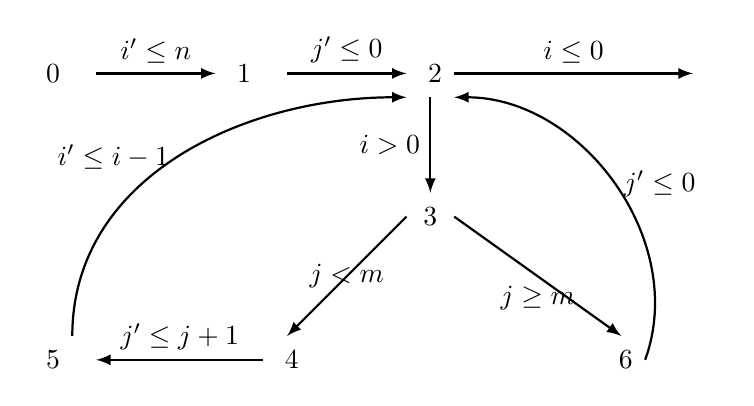
\begin{tikzpicture}[scale=\textwidth/20cm,samples=200]
  \draw[] (-8, 10) circle (0pt) node{{ $0$}};
  \draw[] (-4, 10) circle (0pt) node{{ $1$}};
  \draw[] (0, 10) circle (0pt) node{{ $2$}};
  \draw[] (0, 7) circle (0pt) node{{$3$}};
  \draw[] (-3, 4) circle (0pt) node{{ $4$}};
  \draw[] (-8, 4) circle (0pt) node{{ $5$}};
  \draw[] (4, 4) circle (0pt) node{{ $6$}};
  % Counter Variables
  \draw[] (6, 10) circle (0pt) node {\textbf{$\lex$}};
  %
  % Control Flow Edges:
  \draw[ thick, -latex] (-7, 10)  -- node [above] {$i' \leq n$}(-4.5, 10);
  \draw[ thick, -latex] (-3, 10)  -- node [above] {$j' \leq 0$}(-0.5, 10);
  \draw[ thick, -latex] (0, 9.5)  -- node [left] {$i > 0$} (0, 7.5) ;
  \draw[ thick, -latex] (0.5, 7)  -- node [below] {$ j \geq m $}  (4, 4.5);
  \draw[ thick, -latex] (-7.5, 4.5)  to  [out=90,in=180]  node [left] {$i' \leq i - 1$ }(-0.5, 9.5);
  \draw[ thick, -latex] (4.5, 4)  to  [out=70,in=0]   node [right] {$j' \leq 0 $}(0.5, 9.5);
  \draw[ thick, -latex]  (-0.5, 7) -- node  {$j < m$}  (-3, 4.5) ;
  \draw[ thick, -latex]  (-3.5, 4) -- node [above] {$j' \leq j + 1$}  (-7, 4) ;
  \draw[ thick, -latex] (0.5, 10)  -- node [above] {$i \leq 0$}  (5.5, 10);
  \end{tikzpicture}
  \caption{}
    \end{centering}
    \end{subfigure}
  \caption{
  (a) The Two Paths While Loop Example
    (b) The Abstract Execution Control Flow Graph}
      \label{fig:twoPathsWhile_abscfg}
  \end{figure}
  }
The program in Figure~\ref{fig:twoPathsWhile_abscfg}(a) is an example of two paths loop with different reachability-bounds on the control
locations in different paths.
Its abstract control flow graph is shown in Figure~\ref{fig:twoPathsWhile_abscfg}(b).
The edge $(0 \xrightarrow{i' \leq n} 1)$ on the top tells us the command 
$\clabel{\assign{i}{n}}^0$ is executed with a continuation point $1$, and the
command $\clabel{\assign{j}{0}}^1$ will be executed next.
The annotation $i' \leq 0$ is a difference constraint 
computed by $\absexpr$ over
the expression $n$ in the assignment command $\assign{i}{n}$.
It represents that the value of $i$ is less than or equal to value of $n$ after the
execution of $\clabel{\assign{i}{n}}^0$ and before executing $\clabel{\assign{j}{0}}^1$.
Another example constraint $i' \leq i - 1$ on the edge $5 \xrightarrow{i' \leq i - 1} 2$
describes the execution of
 the command at line $5$, 
$\clabel{\assign{i}{i - 1}}^{5}$. 
The $i'$ on the left side of $i' \leq i - 1$ represents the value of $i$ after the assignment operation,
and the right-hand side $i$ stores the value before the assignment.
The boolean constraint $i \leq 0 $ on the edge $2 \xrightarrow{i \leq 0} \lex$, 
represents the negation of the testing guard $i > 0$
in the $\ewhile$ command with loop header at line $2$.
$2 \xrightarrow{i \leq 0} \lex$ denotes that $i \leq 0$ must hold in order to perform this transition from program point $2$ to
the program exit. 
\end{example}
    \subsection{Loop Refinement}
    \label{sec:refine}
    Three steps:
\begin{enumerate}
  \item It first collects all \emph{simple transition paths}.
  Every \emph{simple transition paths}, $\tpath \in \paths(\absG(c))$ 
  contains only the edges of atomic assignment or guard transitions without interleaving other paths.
  Each of them corresponds to a path in the flatten program in Definition~4.1 in \cite{GulwaniJK09}.
%
    \item \textbf{Rewrite the Program}
    Then it rewrites the program $c$ by rearranging all \emph{simple transition paths} as the syntax in \cite{GulwaniJK09} and preserves the same semantics.
\item \textbf{Refined Program}
Then it computes the 
refined program, $\rprog$ by Algorithm~1 in paper~\cite{GulwaniJK09}.
\\
This step invokes the algorithm REFINE from paper~\cite{GulwaniJK09} and compute the 
refined program $\rprog$ for a program $c$ given the rewritten program as input.
\end{enumerate}

\subsection{Collecting The Simple Transition Path}
We first collect the loop headers $\loopl(c) \subseteq \lvar(c)$ from a program $c$, which is the set of all program points corresponding to the loop headers in program $c$.
\begin{defn}[Loop Headers ($\loopl : \cdom \to \mathcal{P}(\ldom)$)]
  \label{def:loopl}
  \[
  \loopl(c) \triangleq 
  \left\{
    \begin{array}{ll}
      \{\}  & {c} = [{\assign x e}]^{l} \\
      \loopl({c_1}) \cup \loopl({{c_2}})  & {c} = {c_1};{c_2} \\
      \loopl(c_1) \cup \loopl({{c_2}})   & {c} =\eif([\bexpr]^{l}, c_1, c_2) \\
  \loopl(c') \cup \{l\}, &  {c}   = \ewhile ([\bexpr]^{l}, {c}')
  \end{array}
\right.
\]
  \end{defn}
% \begin{defn}[Loop Path]
%   \label{def:looppath}
% A simple transition path
% $\tpath \in \paths(\absG(c))$ for the program $c$, is a path on its abstract transition graph $\absG(c) = (\absV(c), \absE(c))$ with 
% \begin{itemize}
% \item a vertices sequence $(l_0, \ldots, l_n)$, where $l_i \in \absV(c)$ for every $i = 0, \ldots, n$ and
% %
% \item an edge sequence $(e_1, \ldots, e_n)$, where $e_i = (l_{i - 1}, dc_i, l_{i}) \in \absE(c)$ for every $i = 1, \ldots, n$,
% \end{itemize}
% %
% satisfying:
% \begin{itemize}
%   \item $l_i \neq l_j$ for every $i = 0, \ldots, n$ and $j = 0, \ldots, {n - 1}$,
%   \item $l_0$ is either the program point of a loop header or the program entrance ($l_0 = 0$),
%   i.e., $l_0 \in \loopl(c) \cup \{ 0 \}$
%   \item and $l_n$ is either the program point of a loop header or the program exit ($l_n = \lex$),
%   i.e., $l_0 \in \loopl(c) \cup \{ \lex \}$.
% \end{itemize}
% \end{defn}

\begin{defn}[Simple Tansition Path]
  \label{def:tpath}
A \emph{simple transition path}
$\tpath \in \paths(\absG(c))$ for the program $c$, is either a simple cyclic path, which has the same start- and end-point
or a simple path has either different while loop headers, the program entrance or exit as its start- and end-point
without visiting any loop header inside the path.
\\
Specifically, a path $l_0 \xrightarrow{dc_0} l_1 \xrightarrow{dc_1} \ldots l_n \in \paths(\absG(c))$ with the
vertices sequence $(l_0, \ldots, l_n)$, where $l_i \in \absV(c)$ for every $i = 0, \ldots, n$ and
%
the edge sequence $(e_1, \ldots, e_n)$, where $e_i = (l_{i - 1}, dc_i, l_{i}) \in \absE(c)$ for every $i = 1, \ldots, n$,
%
is a \emph{simple transition path} if and only if it satisfies,
\begin{itemize}
  \item $l_i \neq l_j$ for every $i = 0, \ldots, n$ and $j = 0, \ldots, {n - 1}$,
  \item $l_0$ is either the program point of a loop header or the program entrance ($l_0 = 0$),
  i.e., $l_0 \in \loopl(c) \cup \{ 0 \}$
  \item and $l_n$ is either the program point of a loop header or the program exit ($l_n = \lex$),
  i.e., $l_0 \in \loopl(c) \cup \{ \lex \}$,
  \item and $l_i \notin \loopl(c) \cup \{ 0, \lex \}$ for every $i = 1, \ldots, n-1$.
\end{itemize}
\end{defn}

\paragraph{Example.}
$2 \to 3 \to 6 \to 2$ is a transition path on $\absG(\kw{twoPathsWhile}(n, m))$ in Figure~\ref{fig:twoPathsWhile_abscfg}(b).
However, $2 \to 3 \to 6 \to 2 \to 3 \to 4 \to 5 \to 2$ is not a transition path because it is not simple (the program points $2$ and $3$ are visited twice).
In Figure~\ref{fig:threeWhile-overview}(b), $1 \to 2 \to 3 \to 4 \to 5 \to 6$ is not a transition path on $\absG(\kw{threeNestedWhile}(n, m, N))$ because it visits a loop header $3$ inside the path.

\subsection{Rewrite and Refine the Program}
\paragraph{Rewrite the Program}
\begin{algorithm}
  \caption{Program Rewriting $\kw{Rewrite}$}
  \label{alg:alg-refine_rewrite}
  \begin{algorithmic}[1]
    \REQUIRE program $c$
    \STATE finds all $c$'s \emph{simple transition path}s, $\tpath_1, \ldots, \tpath_n \in \paths(\absG(c))$.
    \STATE \textbf{init}: candidate set $W = \{c_1, \ldots, c_n\}$, where $c_i = \tpath_i$ and $i = 1, \ldots, n$
    \STATE \textbf{while} $W.size()> 1$:
    \STATE \quad create $c' = \rpchoose{c_1, \ldots, c_m}$ 
    s.t. $c_i \in W \land c_i[0] = c_j[0] \land c_i[-1] = c_j[-1], i, j = 1, \ldots, m$.
    \\ \quad $W.add(c')$ \qquad $W.remove(c_1, \ldots, c_m)$
    \STATE
    \quad create $c' = \rprepeat(c)$ s.t. $c_i \in W \land c[0] = c[-1] \land c[0] \in \loopl(c)$
    \\ \quad $W.add(c')$, \qquad $W.remove(c)$
    \STATE \quad create $c' = c_1; c_2$ s.t. $c_1, c_2 \in W \land c_1[-1] = c_2[0]$
    \\
    \quad $W.add(c')$ \qquad $W.remove(c_1, c_2)$
    \STATE \textbf{Endwhile}
    \\ $c^T = W[0]$
    \RETURN $c^T$.
\end{algorithmic}
\end{algorithm}
%
Line-2: initialize each candidate $c_i$ with a simple transition path $\tpath_i$.
\\
Line-4: for all the candidates $c_1, \ldots, c_m$ having the same starting and ending vertices, rewrite them into if statement as~\cite{GulwaniJK09}.
\\
Line-5: for every candidate $c'$, if it starts and ends with the same vertex, rewrite it into while loop statement as~\cite{GulwaniJK09}.
\\
Line-6: for every two candidates $c_1, c_2$, if $c_1$ ends with the same vertex as $c_2$'s starting label, rewrite them into sequence statement as~\cite{GulwaniJK09}.
\\
We use simple depth first search strategy computes all the \emph{simple transition path}s satisfying the Definition~\ref{def:tpath} below.
It guarantees that  every $\tpath$ is equivalent to a path $\rho$ in Definition~4.1 of \cite{GulwaniJK09}.

\paragraph{Refined Program}
We implement the algorithm REFINE from paper~\cite{GulwaniJK09} and compute the 
refined program $\rprog$ for a rewritten program $c$.

    \subsection{Path-sensitive Reachability-Bound Analysis}
    \label{sec:psrb}
    Our path-sensitive reachability-bound algorithm relies on the \emph{Abstract Transition Graph}, $\absG(c)$, the \emph{Refined Program}, $\rprog$ and the upper bound invariant of the \emph{Ranking Function} computed previously for the program $c$.
It first requires to compute the new quantities, \emph{Path Reachability-bound} and the \emph{Loop Reachability-bound}, and this section introduces the definition and the following sections describe how we compute them.
%  of \emph{Path Reachability-bound} and the \emph{Loop Reachability-bound}. 

% Given a program $c$ with its \emph{Abstract Transition Graph}, $\absG(c)$ and refined program $\rprog$, our path-sensitive reachability-bound algorithm is presented as follows.

As pre-procedures, we first need to compute the loop bound, $BD(\rprog', c) \in \scexpr(c)$ for every subprogram $\rprog'$ of $c$ in $\rprog$, and use it to estimate the \emph{path local reachability-bound}, $\outinB(\rprog_l, \tpath, c) \in \scexpr(c)$ for each $\tpath$ w.r.t. the sub loop program $\rprog_l$.
\begin{defn}[Loop Bound]
  % \label{def:loopbound}
  For any program $c$ with it refined program $\rprog$,
  the loop bound $BD(\rprog', c) \in \scexpr(c)$ for a subprogram $\rprog'$ of $c$ in $\rprog$ is a upper bound on the iterating times of this program from its enter point to the exit point.
\end{defn}
% 
% Then we compute the \emph{path local reachability-bound}, $\outinB(\rprog_l, \tpath, c) \in \scexpr(c)$ for every sub loop program $\rprog_l$ of $c$ in $\rprog$.
\begin{defn}[Path Local Reachability-bound]
  % \label{def:pathlocalrb}
  Given program $c$ with its refined program $\rprog$ and a simple transition path $\tpath$ in this program, 
  let $l: \rprog_l = \kw{enclosed}(\rprog, \tpath)$ be a sub loop program in $\rprog$,
  then $\tpath$'s \emph{path local reachability-bound} w.r.t. $l: \rprog_l$,  $\outinB(\rprog_l, \tpath, c) \in \scexpr(c)$
  is an upper bound on the execution times of $\tpath$ when executing program $\rprog$.
\end{defn}
Intuitively,
% the local reachability-bound of a \emph{simple transition path},
$\outinB(\rprog_l, \tpath, c)$ bounds the execution times of $\tpath$ when executing its innermost loop program $\rprog_l$.
% and $\rprog$ is the closest loop where $\tpath$ is nested.
For example in the first interleaving pattern $\rprog_1^1$ in Example~\ref{ex:relatedNestedWhileOdd-overview}, 
$4:\rprepeat(\tpath_3)$ is the innermost loop program of $\tpath_3$. So we first compute $m - n$ as its \emph{path local reachability-bound} to bound its iteration times in its closest loop by Section~\ref{sec:pathlocalrb}.
% $4:\rprepeat(\tpath_3)$ is the innermost loop program of $\tpath_1$, $\tpath_2$ and $\tpath_4$.
% We compute the $\frac{m}{4}$ for all the three path $\tpath_1$, $\tpath_2$ and $\tpath_4$ w.r.t. $\rprog_1^1$, as their \emph{path local reachability-bound}.
% $\outinB(1: \rprog_1^1, \tpath_1) = \frac{m}{4}$,
% $\outinB(1: \rprog_1^1, \tpath_2) = \frac{m}{4}$,
% $\outinB(1: \rprog_1^1, \tpath_4) = \frac{m}{4}$,

Next, we define the \emph{loop reachability-bound},
$\lpchB(l: \rprog_l, \tpath, c) \in \scexpr(c)$ for every outer loop program $\rprog_l$ of $\tpath$ in $\rprog$. This quantity aims to precisely bound the iteration numbers of the outer loop $l$,
such that,
during these iterations, the innermost loop $l' = \kw{enclosed(\tpath)}$ is executed, i.e., reached.
\begin{defn}[Loop Reachability-bound]
% \label{def:looprb}
For a program with its refined program $\rprog$ and a simple transition path $\tpath$ in this program, 
let $l: \rprog_l$ be a loop program in $\rprog$,
then $l: \rprog_l$'s \emph{loop reachability-bound} w.r.t. $\tpath$,  $\lpchB(l: \rprog_l, \tpath, c) \in \scexpr(c)$
is the upper bound on iteration numbers of the outside loop $l$,
such that,
during these iterations, the nested loop $l' = \kw{enclosed(\tpath)}$ is entered.
\end{defn}
As introduced in Section~\ref{sec:overview} for Example~\ref{ex:relatedNestedWhileOdd-overview}, $\tpath_3$ has an outer loop program $\rprog_1^1$. Since $L_4$ will be ``entered'' only in the first iteration of $\rprog_1^1$,
we aim to compute $1$ for $\lpchB(\rprog_1^1, \tpath_3, c)$ in Section~\ref{sec:looprb}.
  % and we compute $\lpchB(\rprog_1^1, \tpath_3, c) = 1$. It is tight because the innermost loop of $\tpath_3$ will be ``entered'' only in the first iteration of $\rprog_1^1$.

% Intuitively $\lpchB(l: \rprog_l, \tpath, c) \in \scexpr(c)$
% is the bound on iteration numbers of the outside loop $l$,
% such that,
% during these iterations, the nested loop $l' = \kw{enclosed(\tpath)}$ is executed, i.e., reached.
The \emph{path reachability-bound}, $\inoutB(\rprog, \tpath)$ for each $\tpath$
aims to bound the execution times of $\tpath$ globally during the execution of $c$ and Section~\ref{sec:pathrb} presents the estimating algorithm.
%
\begin{defn}[Path Reachability-bound]
% \label{def:pathrb}
For a program $c$ with its refined program $\rprog$ and a simple transition path $\tpath$ in this program, 
$\tpath$'s reachability-bound, $\inoutB(\rprog, \tpath) \in \scexpr(c)$ is the upper bound on the
execution times of $\tpath$ when executing the $\rprog$.
\end{defn}
% Intuitively, $\inoutB(\rprog, \tpath)$ bounds the execution times of $\tpath$ globally during the execution of $c$.

For our running program in Example~\ref{ex:relatedNestedWhileOdd-overview}, since there isn't nested loop for $\tpath_1, \tpath_2$ and $\tpath_3$, we compute their $\inoutB(\rprog, \tpath) = \frac{m}{4} $, which is the same as their local bound.
While for $\tpath_3$ we compute  the $\inoutB(\rprog, \tpath_3) = \frac{m}{4} \times 1$ by multiplying its local bound with loop reachability bound.
% path is $\tpath_3 = \frac{m}{4} \times 1 = \frac{m}{4} $.

% \paragraph{Program Points Reachability-bound Computation}
% \label{sec:point-psrb}
The \emph{Reachability-bound} for program points is finally computed as follows.
For each program point in a program $c$, $l \in \lvar(c)$,
%  in a program $c$,
its \emph{reachability-bound}, $\psRB(c, l)$ during the execution of $c$ is computed as follows.
%
\begin{defn}[Program Point Reachability-bound Computation]
\label{def:point_psrb}
Given a program $c$ with its \emph{Abstract Transition Graph}, $\absG(c)$ and refined program $\rprog$,
the \emph{reachability bound} of each program point $l \in \lvar(c)$, $\psRB(c, l)$ 
sums up all the path reachability bounds, $\inoutB(\rprog, \tpath)$ over all simple transition paths $\tpath$ that contains the program point $l$.
\[ 
  \psRB(c, l) = 
  \sum
  \left\{ \inoutB(\rprog, \tpath) ~\vert~ \tpath \in \rprog \land 
  l \in \tpath \right\}\footnotemark
\]
$l \in \tpath$ denotes that the program point $l$ is a vertex on $\tpath$ 
and $\tpath \in \rprog$ denotes $\tpath$ is a simple transition path in $\absG(c)$.
\footnotetext{$l \in \tpath$ and $\tpath \in \rprog$, the $\in$ notation is abused to denote
the program point $l$ is a vertex on this path and $\tpath$ is a simple transition path on $\absG(c)$ respectively.}
\end{defn}
$\econfig{\psRB(c, l)}$ is a \emph{reachability-bound} for every program point $l$ in a program $c$.
\begin{thm}[Soundness of the Path-sensitive Reachability-bound Estimation]
\label{thm:pathsensitive_rb_soundness}
For every program ${c}$ and every label $l$ in this program,
$\econfig{\psRB(c, l)}$ is a \emph{Reachability-bound} for $l$ in $c$.
%
{\small
\[
  \begin{array}{l}
    \forall c, c_r \in \cdom, \tpath \in \absG(c), \trace_0 \in \ftdom_0(c),  \trace_r \in \ftdom_0(c_r), \trace \in \tdom, l, l' \in \ldom, \rprog \st 
    \\ \qquad
    \rprog = REFINE(\algrewrite(c))
    \land 
    \rprog = \algrewrite(c_r)
    \land
    \\ \qquad
    \land
    \Big(
    \config{c_r, \trace_0} \rightarrow^* \config{\clabel{\eskip}^{l'}, \trace_0 \tracecat \trace}
    \lor \config{c_r, \trace_0} \uparrow^{\infty} \trace_0 \tracecat \trace 
    \Big)
    \\ \qquad
    \implies \econfig{\psRB(c, l)}(\trace_0) \geq \counter(\trace, l)
  \end{array}.
\]
}
\end{thm}
    \subsection{Loop Reachability-Bound}
    \label{sec:looprb}
    The loop reachability bound is formally defined below. 

\begin{defn}[Loop Reachability Bound]
    \label{def:looprb}
    Loop Reachability Bound
    \begin{equation}
        \label{eq:looprb}
      \lpchB(l: \rprog, \tpath) \triangleq
        \frac{\lpinit(l: \rprog, \tpath) - \rffinal(\tpath)}{\lpnext(l: \rprog, \tpath)}
    \end{equation}
  \end{defn}

  We first compute each component in Equation.~\ref{eq:looprb}
  and solve the computation by SMT solver as follows.
  \\
  1. Compute the ranking function for every transition, $\locbound(\tpath)$ and estimate its maximum value,
  $\varinvar(\locbound(\tpath))$.
  This computation are adopted from \cite{sinn2017complexity} with more details in Section~\ref{sec:rank}.
  \\
  2. Compute the abstract states,  $\lpinit(l: \rprog, \tpath)$,
  $\rffinal(\rprog)$, and $\lpnext(l: \rprog, \tpath)$ using ranking function,
  as in Definition~\ref{def:alg-absstate}.
  \\
  3. Solve the equation using abstract states above and SMT solver.
%
\begin{defn}[Abstract States Computation]
\label{def:alg-absstate}
The abstract states $\lpinit(l: \rprog, \tpath)$, $\lpnext(l: \rprog, \tpath) \in \mathcal{A}_{in}$,
and $\rffinal(\rprog)$ are computed as follows.
\begin{itemize}
   \item 
The loop initial state 
$\lpinit(l: \rprog, \tpath) \in \mathcal{A}_{\lin}$ is symbolic expression as well. 
It describes the abstract initial value of $\tpath$'s ranking function before
any visit of $\tpath$ and during the first execution of $l: \rprog$.
\[
  \lpinit(l: \rprog, \tpath) \triangleq 
  \arg\max_{l_1}\left\{
       \varinvar(y) + v ~\middle\vert~ 
       \begin{array}{l} 
         (l_1, x' \leq y + v, l_2) \in \reset(x) 
         \\
         \land \absinit(\rprog) \leq l_1 \leq \absinit(\tpath)
       \end{array}
     \right\}
    , x = \locbound(\tpath)
  \]
\item
The loop next state 
$\lpnext(l: \rprog, \tpath) \in \mathcal{A}_{\lin}$ 
describes how much $\tpath$'s ranking function
is modified before
the second visit of $\tpath$ but during the second execution of $l: \rprog$.
\footnote{$l' \in \rprog$: the $\in$ notation is abused to denote
the program point $l'$ is a vertex on a path in the program $\rprog$.}
%
\[
  \begin{array}{l}
  \lpnext(l: \rprog, \tpath) \triangleq 
    \begin{array}{l}
  \sum\limits_{(x, \absevent) \in \inc(x) }
  \left\{ 
    \varinvar(y) + v ~\middle\vert~ \absevent = (l', x' \leq y + v, \_) \land  l' \in \rprog 
    \land l' \notin \tpath \right\}
    \\ \qquad 
    - \sum\limits_{(x, \absevent) \in \dec(x) }\left\{ 
      \varinvar(y) + v 
      ~\middle\vert~ \absevent = (l', x' \leq y + v, \_) \land l' \in \rprog \land l' \notin \tpath \right\}
    \end{array}
  \end{array}
  , x = \locbound(\tpath)
  \]
  \item  The \emph{Final State}, $\rffinal(\rprog)$ a conjunction of boolean expressions.
  It is the post-condition
  after the execution of $\rprog$.
\[
    \rffinal(\rprog) \triangleq 
    \bigwedge_{b \in \kw{Guard}(\rprog)}
    \neg b
\]
   $\kw{Guard}(\rprog)$ is the set of all the unique boolean expressions (i.e., the boolean constraints) on this program.
\end{itemize}
\end{defn}

    \subsection{Ranking Function Computation and Estimation}
    \label{sec:rank}
    Three steps:
\begin{enumerate}
    \item It first collects three edge sets for each variable,
  in which the variable increases, decreases and reset respectively.
  \item
  Then, it assigns a symbol $x \in \scvardom$ to the edge on which this symbol decreases as this edge's ranking function.
  \item
  In the last step, it estimates the upper bound invariant on the maximum value of each ranking function recursively.
  In the meantime, it also computes a loop bound path-insensitivity for each loop, which can be used to compute the path reachability-bound later.
  \end{enumerate}

  The algorithm in this step is inspired from the Algorithm.2 in paper~\cite{SinnZV14},
  % which assigns a variable to each edge on which this variable decrease as its ranking function.
  the Algorithm.3 in paper~\cite{ZulegerGSV11},
  and the Definition.25 in Section 4 of paper~\cite{SinnZV17}.
  Algorithm.3 in paper~\cite{ZulegerGSV11} assigns a set of variables to each transition in which these variables decrease as the local bound
  and estimates the maximum value each variable in this set.
  Algorithm.2 in paper~\cite{SinnZV14} assigns a variable to each edge on which this variable decrease as its ranking function
  and then estimates the maximum value for the ranking function.
  The Definition.25 in paper~\cite{SinnZV17}
  assigns each transition with a variable that decreases in this transition, as the local bound and computes the bound similarly.
  %
  \subsection{Collecting Variable Modifications}
  For each variable $x$ in a program $c$, this step computes three edge sets, $\inc(x, c)$, $\dec(x, c)$,
  and $\reset(x, c)$ for $x$.
  Every edge in a set corresponds to a transition in which $x$ is increased,
  %  $\inc(x, c)$,
  decreased
  % $\dec(x, c)$ and 
  or reset
  % $\reset(x, c)$, 
  respectively.
  \\
  $\inc: \cdom \to \vardom \to \mathcal{P}(\absevent) $
  is the set of the edges where the variable increase, 
  %\\
  \[ \inc(x, c) = \left\{ \absevent | \absevent = (l, x' \leq x + v, l') \land \absevent \in \absflow(c) \right\} \]
  %\\
  $\dec: \vardom \to \mathcal{P}(\absevent) $
  is the set of abstract events where the variable decrease,
  %\\
  \[\dec(x, c) = \left\{\absevent| \absevent = (l,  x' \leq x - v, l') \land \absevent \in \absflow(c) \right\}\]
  %\\
  $\reset: \cdom \to \vardom \to \mathcal{P}(\absevent) $ is the set of the abstract events where the variable is reset,
%
  \[\reset(x, c) = \left\{ \absevent| \absevent = (l,  x' \leq y - v, l') \land x \neq y \land \absevent \in \absflow(c) \right\}\]
  Additionally,
  we also compute the reset graph $\resetG(c)$ and the reset chain, $\resetchain(x, c) \in \mathcal{P}(\mathcal{P}(\absevent))$ for every rank $x$.
  The $\resetchain(x, c)$ for every rank $x$ contains all the paths in $\resetG(c)$ that are end at $x$.
  The computation of $\resetG(c)$ and $\resetchain(x, c)$ follows the Definition~20 in~\cite{SinnZV17}.
  \[\resetG(c) = (\resetV(c), \resetE(c))\]
  \[\resetE(c) = \left\{ (x, \absevent, y) ~\vert~ \absevent \in \reset(x, c) \land \absevent = (l, x' \leq y + c, l') \right\} \]
  \[\resetV(c) = \left\{ x ~\vert~ (x, \_, \_) \in \resetE(c) \lor (\_, \_, x) \in \resetE(c) \right\} \]
  In a variable $x$'s reset chain set, $\resetchain(x, c)$, in each chain $(e_0, \ldots, e_m) \in \resetchain(x, c)$
  a variable $x_i$ is reset by another variable $x_{i + 1}$ on edge $e_{i}$
  and $x_{i + 1}$ is reset on edge $e_{i + 1}$ recursively
  for every $i = 0, \ldots, m - 1$.
  $x$ is reset on the first edge $e_0$ of every sequence in $\resetchain(x, c)$.
  {Each edge $e_i$ in a sequence $(e_0, \ldots, e_m) \in \resetchain(x, c)$
  resets a variable $x_i$ by another variable $x_{i + 1}$ such that $x_{i + 1}$
  is reset on edge $e_{i + 1}$ recursively. The first edge $e_0$ of each sequence resets the variable $x$.}
  % 
  \\
  In the following steps, $c$ is omitted in $\inc(x, c)$,
  $\dec(x, c)$ and $\reset(x, c)$ for concise when the reference of a program $c$ is clear in the context.

  \subsection{Assigning The Ranking Function to An Edge}
  For each edge in the transition graph $\absG(c)$ of a program $c$,
  this step assigns the variable that decreases on this edge as the ranking function of this edge.
  This step adopts the local bound computation method in Section 4 of~\cite{SinnZV17} to assign the local bound to each edge,
  formally as follows.
  \begin{defn}[Ranking Function Generatation]
  \label{def:ranking_gen}
  For every edge $\absevent$ in the transition graph $\absG(c)$ of a program $c$,
  its \emph{ranking function/local bound}, $\locbound(\absevent, c)$
  is the variable that decreases on this edge, computed as follows,
  %
  \[ 
\begin{array}{ll}
  \locbound(\absevent, c) \triangleq 1 
  & \absevent \notin SCC(\absG(c))
  \\
  \locbound(\absevent, c) \triangleq x
  & \absevent \in SCC(\absG(c)) \land \absevent \in \dec(x, c) \land  \absevent = (\_, \_ , x' \leq x - v) \\
  \locbound(\absevent, c) \triangleq x
  & \exists \absevent' \in \absG(c), \tpath \in \paths( \absG(c)) \st \absevent, \absevent' \in \tpath \land \locbound(\absevent', c) = x \\
  % \in SCC(\absG(c)) \land \absevent \in \dec(x, c) \land  \absevent = (\_, \_ , x' \leq x - v) \\
  \locbound(\absevent, c) \triangleq x
  & \absevent \in SCC(\absG(c)) \land 
  \absevent  \notin \bigcup_{x \in \vardom} \dec(x, c)
  \land \absevent \notin SCC(\absG(c) \setminus \dec(x, c))\\
  \locbound(\absevent, c) \triangleq \infty
  & o.w..
\end{array}
\]
  $SCC(\absG(c))$ is the set of all the strong connected components of $\absG(c)$.
  \end{defn}
    The first case is straightforward. 
    For the label $l$ which is not in any while loop, 
    the labeled command with the label $l$ will be 
    evaluated at most once. 
    The second and third cases are guaranteed by the \emph{Discussion on Soundness} in Section 4 in~\cite{SinnZV17}.
    The soundness is formalized in Lemma~\ref{lem:local_bound_sound} with proof in Appendix~\ref{apdx:pathinsensitive_rb_soundness}.
  %
  \paragraph{Example}
  In Figure~\ref{fig:relatedNestedWhileOdd-overview}(b), we assign variable $i$ to edge $7 \xrightarrow{i' \leq i - 1} 1$ as ranking.
  If we remove this edge, the edges on $\tpath_2$ and $\tpath_1$ are not in any SCC, so they also have the same ranking.
In the same way, ranking for edges on $\tpath_4$ is $i$ as well and $k$ for them on $\tpath_3$.


  \subsection{Ranking Function Estimation}
  This step estimates the upper bound, $\varinvar(x, c) \in \scexpr(c)$
  on the maximum value for each ranking function  $x \in  \vardom \cup \scvar(c)$.
  \\
  For a program $c$, the \emph{ranking function bound},
  $\varinvar(\locbound(\absevent, c), c)$ is 
  the bound on the maximum value of the ranking function  
  assigned to the edge $\absevent \in \absE(c)$, formally in Definition~\ref{def:ranking_bound}.
  \\
  In order to estimate the maximum value of $\locbound(\absevent, c)$ assigned to edge $\absevent \in \absE(c)$,
  the bound on the iteration times of each corresponding edge, $\absclr(\absevent, c)$ 
  is computed interactively in a path-insensitive manner.
  % \\ 
  % $\varinvar (x, c) \in \scexpr(c)$
  % \\
  % $\absclr(\absevent, c) \in \scexpr(c)$
  \begin{defn}[Ranking Function Estimation]
    \label{def:ranking_bound}
  For a program $c$ and an edge $\absevent \in \absE(c)$,
  the \emph{ranking function bound}, 
  $\varinvar(\locbound(\absevent, c), c)$ for the ranking function $x = \locbound(\absevent, c)$
  of this edge
  is computed as follows,
    \[ 
  \begin{array}{lll}
    \varinvar(x, c) & \triangleq x & x \in \scvar(c) \\
    \varinvar(x, c) & \triangleq \incrs(x, c) + \max\left\{\varinvar(y, c) + v ~\mid~ (l, x' \leq y + v, l') \in \reset(x, c) \right\} & x \notin \scvar(c)
  \end{array}
  \]
  %
  where $\incrs(x, c) \triangleq \sum\limits_{\absevent \in \inc(x, c)}\{\absclr(\absevent, c) \times v ~\mid~ \absevent = (l, x' \leq x + v, l')\}$
  The path-insensitive bound, $\absclr(\absevent, c) \in \scexpr(c)$  on the execution times of the transition $\absevent$, is interactively computed as well as below,
\[ 
\begin{array}{lll}
  \absclr(\absevent, c) 
  & \triangleq \varinvar(\locbound(\absevent, c), c)  &  \\
  & \quad \text{if} ~ \locbound(\absevent, c) \in \scvar(c) & \\
  \absclr(\absevent, c) 
  & \triangleq
    \sum \left\{ \incrs(y, c) | ch \in \resetchain(x, c) \land y \in ch \right\} & \\
    & \quad + 
  \sum\limits_{ch \in \resetchain(x, c)}
  \min \left\{\absclr(\absevent', c) ~\mid~ \absevent' \in ch\right\} \times 
  \big(\varinvar(in(ch), c) 
  + \sum\limits_{(\_, (\_, x' \leq y + v, \_), \_) \in ch} v \big) & \\
  &  \quad \text{if} ~\locbound(\absevent, c) = x \land x \notin \scvar(c) & ,
\end{array}
  \]
 where $in(ch)$ is the first vertex of the reset chain $ch$.
\end{defn}
  %
We also have the soundness of this path-insensitive transition bound. For a program $c$ and an edge $\absevent \in \absE(c)$,
$\absclr(\absevent)$ is a sound upper bound
on the execution times of this transition by paper~\cite{SinnZV17}, formally below in Theorem~\ref{thm:pathinsensitive_rb_soundness} with proof in Appendix~\ref{apdx:pathinsensitive_rb_soundness}.
%
\begin{thm}[Soundness of the Path-insensitive Transition Bound]
  \label{thm:pathinsensitive_rb_soundness}
For each program ${c}$ and an edge $\absevent = (l, \_, \_) \in \absG(c)$, if $l$ is the label of an assignment command,
%  label $l \in \lvar(c)$,
then its \emph{path-insensitive transition bound} $\absclr(\absevent, c)$ 
 is a sound upper bound on 
the execution times of this assignment command in $c$.
  \[
    \begin{array}{l}
      \forall \trace_0 \in \ftdom_0(c), \trace \in \tdom, c \in \cdom, l, l' \in \lvar(c) \st
      \Big( \config{c, \trace_0} \rightarrow^{*} \config{\clabel{\eskip}^{l'}, \trace_0 \tracecat \trace} 
        \lor  \config{c, \trace_0} \uparrow^{\infty} \trace_0 \tracecat \trace \Big)
       \\ \qquad \qquad
       \implies
       \exists \absevent = (\_, l, \_) \in \absflow(c) \land
      \counter(\trace, l) \leq \econfig{\absclr(\absevent, c)}(\trace_0)
    \end{array}
  \]
\end{thm}
%
\paragraph[example]{Example.}
% \todo{The w example}
Using this ranking function based approach, we first find the ranks for every transition,
$\locbound(0 \to 1) = 1$,
$\locbound(1 \to \lex) = 1$,
$\locbound(1 \to 2) = i$,
$\locbound(2 \to 3) = i$,
$\locbound(3 \to 4) = i$,
$\locbound(4 \to 5) = k$,
$\locbound(5 \to 4) = k$,
$\locbound(4\to 6) = \locbound(6 \to 7) = \locbound(7 \to 1) = i$,
and $\locbound(2 \to 8) = \locbound(8 \to 1) = i$,
Then we estimate the upper bound invariant for the ranking function $i$ and $k$ by computing the transition bound in the same time.
We get $\varinvar(i, c) = n$ and $\varinvar(k, c) = m$.
While the transition bound for each transition is the same as the upper bound invariant of its ranking function.
They are loose and path-insensitive. 

Specifically, in Example~\ref{ex:relatedNestedWhileOdd-overview}, the ranking $i$ is reset by $n$ at edge $0 \to 1$ and 
$k + m$ at edge $6 \to 7$ and $k$ is assigned value $i - m$ at edge $3 \to 4$. Through reset chain graph (which we do not fully presented but can be found in the Definition~20 in~\cite{SinnZV17}), we estimate a symbolic value $n$ for both ranking variable $i$ and $k$.
Interactively, iteration bounds for all the edges in this loop are $n$ as well path-insensitively.
    \subsection{Reachability Bound Computation}
    \label{sec:alg-rb}
    \subsection{Path Global Reachability-Bound}
\label{sec:pathrb}
We first compute $\kw{enclosing}(\rprog)$, which is the set containing \text{all the loops $l:\rprog$ which are nested inside } $\rprog$.
\\
Then, the path global reachability-bound, $\inoutB(\rprog, \tpath)$ for a \emph{simple transition path} $\tpath$ is computed as in Definition~\ref{def:pathrb}.
%
\begin{defn}[Path Reachability-Bound]
  \label{def:pathrb}
\[
  \begin{array}{rcl}
    \inoutB(\tpath, \tpath) & \triangleq & 1  \\
    \inoutB(\tpath', \tpath) & \triangleq & \highlight{0} \qquad \text{if } \tpath' \neq \tpath\\
    \inoutB(\rprog_1;\rprog_2, \tpath) & \triangleq & \inoutB(\rprog_1, \tpath) + \inoutB(\rprog_2, \tpath) \\
    \inoutB(l: \rprog', \tpath) & \triangleq & 
    \highlight{\outinB(\rprog', \tpath), \qquad \text{if } l = \kw{enclosed}(\tpath)}
    \\
    &  \triangleq & 
   0, \qquad \qquad \qquad \quad ~~ \text{if }  \kw{enclosed}(\tpath) \notin \kw{enclosing}(\rprog')
    \\
    &  \triangleq & 
    \highlight{
      \lpchB(l:\rprog', \tpath ) }
    \highlight{\times \max\limits_{l = \kw{enclosed}(l':\rprog'')}
   \{\inoutB(l':\rprog'', \tpath)\} } \footnotemark, o.w. \\
    \inoutB(\rpchoose{\rprog_1, \ldots, \rprog_m }, \tpath) & \triangleq 
    & \max\left\{ \inoutB(\rprog_1, \tpath), \ldots, \inoutB(\rprog_m, \tpath) \right\} 
    \\
    \inoutB(\rprepeat(\rprog'), \tpath) & \triangleq & \outinB(\rprepeat(\rprog'), \rprog) \times \inoutB(\rprog', \tpath)\\
    &  & \text{this case will never be matched}
    \end{array}
  \]
  \end{defn}
\footnotetext{There is only one non-zero $\inoutB(l':\rprog'', \tpath)$ where $\tpath \in \rprog''$, all the others $\inoutB(l':\rprog'', \tpath)$ where $\tpath \notin \rprog''$ equal to $0$}%
We show that $\inoutB(\rprog, \tpath)$ bounds the execution times of $\tpath$ during the execution of $\rprog$

We show the \emph{path reachability-bound} of the simple transition path $\tpath$ in a refined program $\rprog$ is a sound upper bound of its execution times when executing the program in Lemma~\ref{lem:pathrb-sound}, with the proof in \highlight{Appendix~\ref{apdx:pathrb-sound}}.
\begin{lem}[Soundness of the Path Reachability-Bound]
  \label{lem:pathrb-sound}
  For any program with its refined program $\rprog$ and a simple transition path $\tpath$ in this program,
  the execution times of $\tpath$ when executing the $\rprog$ is bounded by $\inoutB(\rprog, \tpath)$.
  \[
    \begin{array}{l}
    \forall c \in \cdom, \tpath \in \absG(c), \trace_0 \in \tdom_0(c), \trace \in \tdom, \rprog \st 
    \rprog = REFINE(c)
    \land
    \config{c, \trace_0} \to^* 
    \config{{\eskip, \trace_0 \tracecat \trace}}
    \\ \qquad
    \implies
    \config{\inoutB(\rprog, \tpath)}(\trace_0) \geq \counter(\vtrace, L(\tpath)).
    \end{array}
    \]
  \end{lem}

\subsection{Program Points Path-sensitive Reachability-Bound}
\label{sec:point-psrb}
For each program point in a program $c$, $l \in \lvar(c)$,
%  in a program $c$,
its \emph{path-sensitive reachability-bound}, $\psRB(c, l)$ is a sound upper bound on the executing times of $l$ during the execution of $c$.
%
 \begin{defn}[Path-Sensitive Reachability Bound]
  \label{def:point_psrb}
  Given a program $c$ with its \emph{Abstract Transition Graph}, $\absG(c)$ and refined program $\rprog$,
  the \emph{reachability bound} of each program point $l \in \lvar(c)$, $\psRB(c, l)$ 
  sums up all the path reachability bounds, $\inoutB(\rprog, \tpath)$ over the $\tpath$ which contains the program point $l$.
  \[ 
    \psRB(c, l) = 
    \sum\limits_{\tpath \in \rprog \land 
  l \in \tpath} 
  \inoutB(\rprog, \tpath)
  \]
  $l \in \tpath$ denotes that the program point $l$ is a vertex on $\tpath$ 
  and $\tpath \in \rprog$ denotes $\tpath$ is a simple transition path of program $c$.
 \end{defn}
We show that $\config{\psRB(c, l)}$ is a \emph{Reachability-Bound} for every program point $l$ in a program $c$ with proof in Appendix~\ref{apdx:psrb-sound}.
\begin{thm}[Soundness of the Path-sensitive Reachability Bound Estimation]
    \label{thm:pathsensitive_rb_soundness}
  For every program ${c}$ and every label $l$ in this program,
  $\config{\psRB(c, l)}$ is a \emph{Reachability-Bound} for $l$ in $c$.
  %
  \[
    \forall c \in \cdom, \trace_0 \in \tdom_0(c), \trace \in \tdom \st 
    \config{{c}, \trace} \to^{*} \config{\eskip, \trace_0 \tracecat \vtrace} 
    \implies \config{\psRB(c, l)}(\trace_0) \geq \counter(\vtrace, l) 
    \]
  \end{thm}



\section{Examples and Experimental Results}
\label{sec:example}

\section{Related Work}
% % \subsection{Cost Analysis}

\paragraph*{Program Model.}
The semantics model mainly inspired from~\cite{Cousot19a} and~\cite{Cousot19}.
The program abstraction and the abstraction transition graph are inspired from~\cite{SinnZV17}.

There are many other program abstraction techniques, but not efficient and accurate enough.

\paragraph{Type-Based Static Cost Analysis.}
\paragraph{Program Cost Analysis.}
The works in analyzing the program complexity~\cite{GustafssonEL05, HumenbergerJK18} only focus on estimating 
the overall complexity 
by inferring the bounds on the loop iteration numbers.
Similarly, the algorithm of computing a program's worst-case resource cost
such as~\cite{BrockschmidtEFFG16, AlbertAGP08, AliasDFG10, Flores-MontoyaH14} reason the worst-case running time and resource cost of the program's entire execution as well.

The CofloCo~\cite{Montoya17, Flores-MontoyaH14, Flores-Montoya16},

The loop bound analysis algorithm in~\cite{LuCT21} works well in but not in multi-paths loops.
\paragraph{Loop Summarization and Termination.}
Termination~\cite{FalkeKS12, FalkeKS11},
Loop summarization and invariant generate~\cite{HumenbergerJK18}.
Invariant Generation Through Ranking functions~\cite{AliasDFG10} for multipath loops.
Closed-form loop summarization techniques~\cite{KincaidBCR19} which can help to improve the accuracy of the path refinement.
Non-linear loop summarization techniques~\cite{KincaidCBR18} we plan to extend in the future.
Advanced loop summarization considering recurrence in~\cite{BreckCKR20}.
\paragraph{Path Refinement.}
\cite{GulwaniJK09}
Path refinement algorithm we are using.
\cite{SinnZV14}
The contextualization path refinement algorithm, based on the loop termination techniques in~\todo{}.
\cite{CyphertBKR19}
Advanced path refinement techniques we plan to extend in the future.


\section{Conclusion and future works}


\subsubsection*{Acknowledgements}
Acknowledgments is at the end of the paper, preceded by an unnumbered run-in heading (i.e.
3rd-level heading).

%
% ---- Bibliography ----
%
% BibTeX users should specify bibliography style 'splncs04'.
% References will then be sorted and formatted in the correct style.
%
\bibliographystyle{splncs04}
\bibliography{main}
%

\end{document}
